\documentclass[11pt]{article}
\usepackage[margin=1in]{geometry}
\usepackage{amsmath,amssymb,amsfonts}
\newcommand{\ket}[1]{\left|#1\right\rangle}
\usepackage{xcolor}
\usepackage{tcolorbox}
\usepackage{enumitem}
\usepackage{booktabs}
\usepackage{hyperref}
\usepackage{tikz}
\usetikzlibrary{arrows.meta,positioning}
\tcbuselibrary{skins,breakable}

% ---- All boxes are pure black/white/gray -- safe for grayscale printing.
% Distinguished by title wording and border weight only, never by color hue.
\newtcolorbox{plain}[1][]{colback=black!2, colframe=black, boxrule=0.4pt, arc=1pt, breakable, left=6pt, right=6pt, top=4pt, bottom=4pt, title={\textsc{In Plain English}},#1}
\newtcolorbox{eqmeaning}[1][]{colback=black!6, colframe=black, boxrule=1pt, arc=1pt, breakable, left=6pt, right=6pt, top=4pt, bottom=4pt, title={\textsc{What This Equation Is Really Saying}},#1}
\newtcolorbox{ifnot}[1][]{colback=white, colframe=black, boxrule=0.4pt, arc=1pt, breakable, left=6pt, right=6pt, top=4pt, bottom=4pt, title={\textsc{If This Term Were Missing}},#1}
\newtcolorbox{takeaway}[1][]{colback=black!10, colframe=black, boxrule=1.4pt, arc=1pt, breakable, left=6pt, right=6pt, top=4pt, bottom=4pt, title={\textsc{Takeaway}}, #1}
\newtcolorbox{simuse}[1][]{colback=black!4, colframe=black, boxrule=0.4pt, arc=1pt, breakable, left=6pt, right=6pt, top=4pt, bottom=4pt, title={\textsc{Why This Matters for the Simulation}}, #1}
% ---- Flowchart building blocks: real TikZ boxes with arrows attached
% directly to them (not floating text arrows that can be orphaned by a
% line-wrap). Longer chains snake: row 1 left-to-right, row 2 right-to-left
% below it, connected by a vertical arrow -- like reading a printed page.
\tikzset{
  fbox2/.style={draw=black, thick, rounded corners=2pt, align=center, font=\small, inner sep=5pt, minimum height=10mm, minimum width=3.4cm, text width=3.2cm},
  farr/.style={-{Latex}, thick}
}

\title{\bfseries A Complete, Plain-English Walkthrough of\\
``Harnessing Rydberg Atomic Receivers:\\ From Quantum Physics to Wireless Communications''}
\author{Study companion --- deep-dive edition, no background assumed}
\date{}

\begin{document}
\maketitle
\tableofcontents
\newpage

% ============================================================
\section{The Aim of the Paper, in One Paragraph}
% ============================================================
Normal radios use an antenna: a piece of metal that a radio wave physically shakes electrons in, producing a current. This paper proposes replacing that metal antenna with a \textbf{cloud of specially-excited atoms} (called Rydberg atoms) floating in a small glass cell. These atoms are so sensitive to electric fields that even a very weak radio wave changes how they behave. The paper never looks at the radio wave directly with an electrical circuit --- instead, it shines two laser beams through the atom cloud and watches how much laser light comes out the other side. The radio wave's presence changes that laser light in a very specific, readable way. The paper builds the complete math describing that process, then asks: if we used this atom-cloud ``receiver'' in an actual wireless communication link, how good would it be? It compares two versions of this atomic receiver against a normal radio receiver, using the yardsticks engineers always use: signal-to-noise ratio (SNR), channel capacity, and symbol error rate (SER).

\begin{plain}
Instead of listening to a radio wave with an antenna wire, you are reading a radio wave's effect on a candle flame's flicker pattern, by watching the candle through a camera. The atoms are the candle; the two lasers are how you illuminate and watch it; the paper is the rulebook for translating flicker patterns back into bits of data.
\end{plain}

\section*{The Complete Journey of a Bit: From Source to Recovery}
Before any equations, walk through the \emph{entire} path one bit takes, start to finish, in plain language. Every later part of this document zooms into one link of this exact chain in full mathematical detail --- this section is the map.

\paragraph{1. At the source: bits become a symbol.}
Data starts as plain 0s and 1s. Before transmission, bits are grouped into small chunks and mapped onto a \textbf{symbol} $x$ --- one point picked from a fixed, agreed set of possible values called a \textbf{constellation}. With 8-QAM, every group of 3 bits ($2^3=8$) selects one of 8 symbols, each carrying both an amplitude and a phase. With 8-PAM (used by the LO-free receiver, since it can only ever measure amplitude), every group of 3 bits selects one of 8 amplitude levels only. This $x$ is exactly the $x$ that appears in every equation in this document.

\paragraph{2. Before the Tx antenna: the symbol becomes a real RF wave.}
$x$ is a number, not yet a physical signal. The transmitter's electronics use it to set the amplitude and phase of a real radio wave, $E_{RF}=A_{RF}\cos(2\pi f_{RF}t+\phi_{RF})$, with $A_{RF},\phi_{RF}$ set directly by $x$. This is ordinary modulation --- nothing atomic-physics-specific has happened yet.

\paragraph{3. Between Tx and Rx: free-space propagation.}
The wave leaves the transmit antenna and spreads out, weakening with distance exactly like any radio wave (Eq.~10, $P_{Rx}=P_{Tx}G_{Tx}\eta_0/4\pi d^2$). By the time it arrives, its power has dropped from $P_{Tx}$ to $P_{Rx}$, but $x$ itself is still intact in the wave's amplitude/phase (real channels also pick up fading $h$ and background noise $n_{BGN}$ along the way).

\paragraph{4. At the receiver: no metal antenna --- atoms instead.}
This is where the Rydberg receiver diverges completely from an ordinary radio. The arriving field does not induce a current in a wire; it reaches directly into the vapor cell and drives the $\ket3\to\ket4$ transition. This IS the entire ``antenna'' step here: a field, present in space, coupling to atoms.
\begin{itemize}[nosep]
\item \textbf{LO-free path}: the RF field alone drives the transition, splitting the EIT window into two peaks separated by $\Omega_{RF}$. $x$ is now encoded as \emph{a gap between two optical peaks}.
\item \textbf{LO-dressed path}: a second, always-on LO field joins in. The two fields beat together, and $x$ (amplitude \emph{and} phase) ends up encoded as \emph{a slow oscillation} in the atoms' optical response, repeating once every beat period $1/\Delta f$.
\end{itemize}

\paragraph{5. Inside the atoms: field becomes optical absorption.}
The driven atoms settle into a steady quantum state $\rho_{21}$, which sets $\chi=C_0\rho_{21}$, which sets exactly how much probe laser gets absorbed, $P_{out}=P_{in}e^{-k_pL\Im(\chi)}$. At this point $x$ has been fully converted from ``a radio wave's amplitude/phase'' into ``how bright the transmitted probe beam is'' --- a purely optical quantity now.

\paragraph{6. At the photodetector: light becomes current.}
The probe beam, carrying $x$'s information as a brightness/timing pattern, hits a photodiode, which converts optical power directly into an electrical photocurrent $I_{AC}=D\times(\text{optical signal})$. This is the first point in the whole chain where the signal is an ordinary electrical current, same as the very last stage of a conventional radio receiver.

\paragraph{7. Through the electronics: amplification and noise.}
This weak photocurrent becomes a power ($P=I^2R_L$), then gets amplified (LNA, gain $G_{LNA}$). At every stage, real noise piles on: background noise picked up before the atoms, photon shot noise from the light itself, thermal noise from the electronics. The final observed quantity ($z$ for LO-free, $z^{LO}$ for LO-dressed) is $x$, scaled by the receiver's overall gain, plus all this accumulated noise.

\paragraph{8. Recovery: noisy observation back to a symbol estimate.}
LO-free: a lock-in amplifier reads the AT-splitting gap ($z$, amplitude-only) and converts it back to an estimated field amplitude. LO-dressed: the photocurrent is Fourier-analyzed at $\Delta f$, recovering both an estimated amplitude \emph{and} phase.

\paragraph{9. The decision: nearest-neighbor detection.}
The receiver compares this noisy estimate against every possible symbol in the known constellation and picks whichever is closest. Call this decision $\hat x$ --- the receiver's final guess.

\paragraph{10. SER: did we get it right?}
Compare $\hat x$ against the $x$ that was actually sent. Match = correct; mismatch = one symbol error. Repeating this over many symbols and counting mismatches gives the \textbf{Symbol Error Rate (SER)} --- the number Fig.~9's curves plot. Every equation in Parts III--IX of this document is working out, in full detail, one specific link of this ten-step chain.

\begin{center}
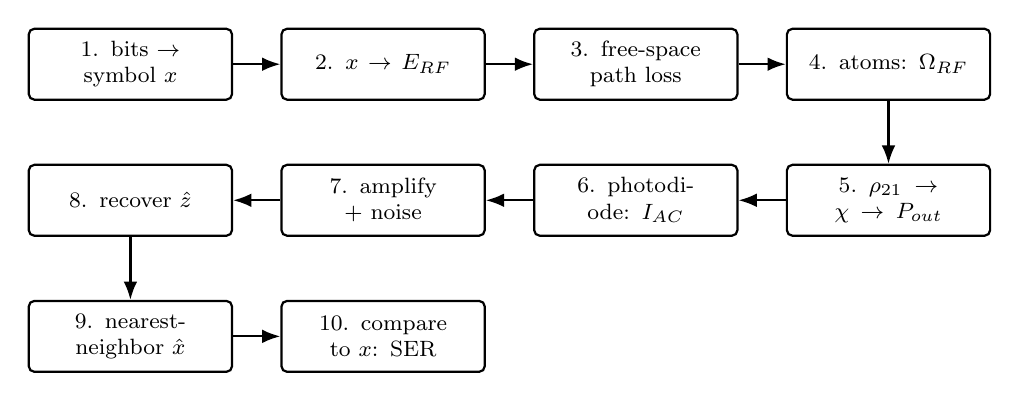
\begin{tikzpicture}[
  bjbox/.style={draw=black, thick, rounded corners=2pt, align=center, font=\footnotesize, inner sep=4pt, minimum height=9mm, minimum width=2.5cm, text width=2.3cm},
  bjarr/.style={-{Latex}, thick}
]
\node[bjbox] (b1) {1. bits $\to$ symbol $x$};
\node[bjbox, right=6mm of b1] (b2) {2. $x\to E_{RF}$};
\node[bjbox, right=6mm of b2] (b3) {3. free-space path loss};
\node[bjbox, right=6mm of b3] (b4) {4. atoms: $\Omega_{RF}$};
\node[bjbox, below=8mm of b4] (b5) {5. $\rho_{21}\to\chi\to P_{out}$};
\node[bjbox, left=6mm of b5] (b6) {6. photodiode: $I_{AC}$};
\node[bjbox, left=6mm of b6] (b7) {7. amplify + noise};
\node[bjbox, left=6mm of b7] (b8) {8. recover $\hat z$};
\node[bjbox, below=8mm of b8] (b9) {9. nearest-neighbor $\hat x$};
\node[bjbox, right=6mm of b9] (b10) {10. compare to $x$: SER};
\draw[bjarr] (b1) -- (b2);
\draw[bjarr] (b2) -- (b3);
\draw[bjarr] (b3) -- (b4);
\draw[bjarr] (b4) -- (b5);
\draw[bjarr] (b5) -- (b6);
\draw[bjarr] (b6) -- (b7);
\draw[bjarr] (b7) -- (b8);
\draw[bjarr] (b8) -- (b9);
\draw[bjarr] (b9) -- (b10);
\end{tikzpicture}
\end{center}

\subsection*{How to read the rest of this document}
Every idea from here on is broken down the same way: a \textbf{``What does X mean?''} question answered in plain bullets first; a box titled \textsc{What This Equation Is Really Saying}; a boxed flowchart showing where that piece sits in the chain above; a box titled \textsc{Why This Matters for the Simulation}; and a box titled \textsc{Takeaway} closing out each major topic.

\newpage
% ============================================================
\section{Part I --- Prerequisites, One Concept at a Time}
% ============================================================

\subsection*{What is an energy level?}
\begin{itemize}
\item An atom's electron cannot sit at just any energy --- only at specific, fixed amounts, like steps on a staircase rather than a smooth ramp.
\item Each fixed amount is called an \textbf{energy level} (sometimes called a ``state''). The lowest one is the \textbf{ground state}; anything higher is an \textbf{excited state}.
\item An atom moves from one energy level to another only by absorbing or releasing exactly the right amount of energy --- usually as a photon of light of exactly the right color.
\item This paper uses four energy levels, and calls them $\ket{1}$ (lowest/ground) up to $\ket{4}$ (highest).
\end{itemize}
\begin{plain}
Think of a building where the elevator only stops on floors 1, 2, 3, and 4 --- never in between. To get the electron from floor 1 to floor 2, you have to hand it exactly the right amount of ``elevator fuel'' (photon energy). Too little or too much and nothing happens.
\end{plain}
\begin{takeaway}
Energy levels are the fixed floors an atom's electron can occupy. Everything in this paper is about controlling and reading out which floor(s) the electron effectively occupies, using light.
\end{takeaway}

\subsection*{Why Rydberg atoms specifically?}
\begin{itemize}
\item A ``Rydberg atom'' is an ordinary atom (Cesium here) with its outer electron pushed to an extremely high energy level --- so high that the electron orbits very far from the nucleus.
\item The levels used are $47D_{5/2}$ and $48P_{3/2}$; the numbers 47 and 48 tell you how far out that electron is (a normal, un-excited electron would be at level 6 or so).
\item Because the electron sits so far away, the atom becomes very easy to electrically distort --- a tiny outside electric field can noticeably tug the electron off-center.
\item This is why Rydberg atoms react to even extremely weak radio waves: their electron is, physically, an oversized target that is easy to push around.
\end{itemize}
\begin{takeaway}
Rydberg atoms are used simply because they are naturally, physically hyper-sensitive to electric fields --- this is a property of the atom itself, not something engineered by circuitry.
\end{takeaway}

\subsection*{What is a laser doing to the atom (resonance and Rabi frequency)?}
\begin{itemize}
\item A laser is light of one precise color (frequency).
\item If that color exactly matches the energy gap between two levels, the laser is \textbf{on resonance} with that pair of levels, and the electron starts flipping back and forth between the two levels over and over.
\item \textbf{Rabi frequency} $\Omega$ is simply how fast that back-and-forth flipping happens.
\item A stronger laser (or a stronger field, for the RF case) drives the flipping faster, which means a bigger $\Omega$.
\end{itemize}
\begin{plain}
Push a kid on a swing steadily and in-time, and they swing back and forth at some rate. That rate is the Rabi frequency. Push harder (or more precisely) and the swinging speeds up.
\end{plain}
\begin{takeaway}
$\Omega$ (Rabi frequency) is not a color or a location --- it is a \emph{rate}: how fast the atom's population is being driven back and forth between two levels by whatever laser or field is coupling them.
\end{takeaway}

\subsection*{What is detuning?}
\begin{itemize}
\item \textbf{Detuning} $\Delta$ measures how far off-color your laser (or field) is from the exact energy gap.
\item $\Delta = 0$ means perfectly on-resonance --- the laser matches the gap exactly.
\item A large $|\Delta|$ means the laser is ``singing the wrong note'' for that transition, and barely drives it at all.
\end{itemize}

\subsection*{What is decay rate, and why does it create a linewidth?}
\begin{itemize}
\item Excited atoms do not stay excited forever. Eventually the electron falls back down on its own, releasing a photon in a random direction. This is called \textbf{spontaneous emission}.
\item How fast this happens is the \textbf{decay rate} $\gamma$ --- a bigger $\gamma$ means a shorter-lived excited level.
\item Because a short-lived level doesn't ``sit still'' in energy for very long, it isn't perfectly sharp either --- it has a small blur in its exact energy, called the \textbf{linewidth}. Short lifetime = big blur = wide linewidth (this is a basic consequence of the quantum uncertainty between time and energy).
\end{itemize}
\begin{takeaway}
$\gamma$ controls two things at once: how fast population leaks out of a level, and how blurry/wide that level's energy is when you try to measure it optically.
\end{takeaway}

\subsection*{What does the ``transparency window'' mean?}
\begin{itemize}
\item In Electromagnetically Induced Transparency (EIT), atoms that would normally absorb the probe laser become transparent when the probe and coupling lasers are tuned correctly together.
\item This creates a \textbf{window} in the absorption spectrum: a narrow frequency range where the probe beam passes through with very little loss, sitting right in the middle of what would otherwise be an absorbing region.
\item That window is exactly where the RF signal gets encoded into the probe transmission --- the whole receiver only works because this window exists and can be watched.
\item Physically: it is like carving out a narrow ``channel'' in the atomic absorption curve, and that channel is where information is allowed to flow through.
\end{itemize}
\begin{plain}
Two people singing exactly opposite notes so precisely that their sound cancels and you hear silence at that one note, even though either one alone would be audible --- EIT is that same kind of destructive-interference silence, but for light absorption instead of sound.
\end{plain}
\begin{takeaway}
The transparency window is not a side-effect --- it is the entire reason this receiver design is possible. No window, no readable signal.
\end{takeaway}

\subsection*{What is a Lorentzian, and what do HWHM/FWHM mean?}
\begin{itemize}
\item If you scan a laser's color across a resonance and plot how strongly the atom responds, you get a bump-shaped curve. The specific bump shape that shows up in this kind of physics is called a \textbf{Lorentzian}:
\[
\Lambda(a,b) = \frac{b^2}{b^2+a^2}
\]
\item $a$ = how far off-resonance you currently are. $b$ = a fixed number describing how wide the bump is.
\item \textbf{HWHM} (Half-Width at Half-Maximum) = distance from the peak's center to the point where the bump has dropped to half its peak height. This is exactly the $b$ above.
\item \textbf{FWHM} (Full-Width at Half-Maximum) = twice the HWHM --- the total width measured at half-height, on both sides.
\end{itemize}
\begin{plain}
Picture a bell-shaped hill. HWHM is ``how far do I walk from the summit before the hill drops to half its height.'' FWHM is that same distance on both sides added together --- how fat the hill is at half-height.
\end{plain}

\subsection*{What is the density matrix, and what does $\rho_{21}$ actually represent?}
\begin{itemize}
\item For a system with several energy levels, physicists track a grid of numbers called the \textbf{density matrix} $\rho$.
\item The diagonal entries ($\rho_{11},\rho_{22},\dots$) tell you \emph{how much population} (probability) sits in each level right now.
\item The off-diagonal entries (like $\rho_{21}$) track something subtler: \textbf{coherence} --- whether the atom is in a clean, laser-driven superposition between two levels, or whether that link has been scrambled by decay/noise.
\item $\rho_{21}$ is the single most important number in the entire paper: it is what actually gets converted into optical absorption and read out at the very end of the physical chain.
\end{itemize}
\begin{plain}
$\rho_{22}$ answers ``what fraction of atoms are currently in level 2.'' $\rho_{21}$ answers a different question: ``how cleanly are levels 1 and 2 still cooperating together, in a coherent quantum-mechanical sense, rather than each doing their own separate thing.''
\end{plain}
\begin{takeaway}
Everything downstream in this paper --- $P_{out}$, SNR, capacity, SER --- is, at bottom, just different ways of extracting and using the single complex number $\rho_{21}$.
\end{takeaway}

\subsection*{What is susceptibility, and what is a dipole moment?}
\begin{itemize}
\item \textbf{Susceptibility} $\chi$ measures how strongly a material bends or absorbs light passing through it. Large $\Im(\chi)$ = strongly absorbing; small $\Im(\chi)$ = nearly transparent.
\item In this paper $\chi \propto \rho_{21}$ directly --- so ``how much light gets through'' is a direct window onto the atoms' internal quantum coherence.
\item \textbf{Dipole moment} $\wp$ of a transition measures how strongly that pair of levels ``grabs onto'' an electric field. A huge dipole moment (which Rydberg transitions have) means even a tiny field produces a large Rabi frequency $\Omega$ --- this is the actual physical source of Rydberg atoms' sensitivity.
\end{itemize}

\subsection*{Quick reference: a few more terms you'll meet later}
These aren't needed yet, but they show up without re-explanation from Part IV onward, so define them once here.
\begin{itemize}[nosep]
\item \textbf{dBm}: a unit of power on a logarithmic scale, referenced to 1 milliwatt. $P_{\text{dBm}}=10\log_{10}(P_{\text{watts}}/10^{-3})$. $0$dBm$=1$mW, $-90$dBm is an extremely small power ($10^{-12}$W) --- used throughout for the background noise level.
\item \textbf{Fourier transform / spectrum}: any wiggly signal that repeats over time can be broken down into a sum of pure, single-frequency tones. The Fourier transform tells you how much of each frequency is present. ``The amplitude of the spectrum at $\Delta f$'' just means ``how strong is the pure tone at frequency $\Delta f$ inside this signal.''
\item \textbf{Responsivity} ($D$, units A/W): how many amps of electrical current a photodiode outputs per watt of light it receives. A simple conversion factor between the optical and electrical worlds.
\item \textbf{Constellation}: the fixed, agreed-upon set of possible symbol values a transmitter is allowed to send (e.g.\ 8 points for 8-QAM/8-PAM). The receiver's whole job is to figure out which one point was sent.
\item \textbf{Antenna gain} ($G$, units dBi): how well an antenna focuses its power in a particular direction compared to a hypothetical antenna that radiates equally in all directions. Higher gain = more focused = stronger signal in that direction, weaker elsewhere.
\end{itemize}

\newpage
% ============================================================
\section{Part II --- The Physical Setup: Why Two Lasers, Why This Shape}
% ============================================================

\subsection*{What is each energy level actually for?}
\begin{center}
\begin{tabular}{@{}cll@{}}
\toprule
Level & Cesium state & Role \\
\midrule
$\ket{1}$ & $6S_{1/2}$ & Ground state --- where almost all atoms start \\
$\ket{2}$ & $6P_{3/2}$ & First excited level, reached by the \textbf{probe} laser \\
$\ket{3}$ & $47D_{5/2}$ & Rydberg level, reached by the \textbf{coupling} laser \\
$\ket{4}$ & $48P_{3/2}$ & A second, nearby Rydberg level, reached only by the \textbf{RF field} \\
\bottomrule
\end{tabular}
\end{center}

\subsection*{Why two lasers, and why do we only ever look at the probe laser afterward?}
\begin{itemize}
\item The \textbf{probe laser} connects $\ket{1}\to\ket{2}$. It is weak, and its whole job is to be a \emph{measurement beam}: shine it through the cell and measure how much survives out the other side, on a photodetector. This transmitted probe power is $P_{out}$ --- the one quantity the entire readout chain is built around.
\item The \textbf{coupling laser} connects $\ket{2}\to\ket{3}$. Its job is not to be measured --- its job is to \emph{prepare} the special quantum state that opens the EIT transparency window, so the probe beam's transmission becomes exquisitely sensitive to whatever is happening at the Rydberg level $\ket{3}$.
\item We never put a detector on the coupling laser; it only sets up the conditions, and its own transmitted power carries no useful information here.
\end{itemize}
\begin{ifnot}
Without the coupling laser, the atoms would just absorb the probe laser normally (a plain two-level absorption line): no transparency window, no way to sense the Rydberg level, and therefore no way to sense the RF field at all.
\end{ifnot}

\subsection*{How does the RF field become visible: Autler--Townes (AT) splitting}
\begin{itemize}
\item Bring in the RF field, driving $\ket{3}\to\ket{4}$. Driving a transition strongly enough physically splits that level's energy into two ``dressed'' levels --- a standard quantum effect.
\item Since the EIT transparency window was pinned to the location of level $\ket{3}$, splitting $\ket{3}$ in two also splits the transparency window into two.
\item You now see \textbf{two} narrow transparency peaks instead of one, and the gap between them is set directly by the RF field's own Rabi frequency:
\[
\Delta\nu = \frac{\Omega_{RF}}{2\pi}\quad\text{(scanning the coupling laser)}
\]
\end{itemize}
\begin{eqmeaning}
Whatever gap you physically measure between the two transparency peaks IS the RF Rabi frequency, directly, with no fitting or calibration mystery in between. Measuring a frequency gap on an optical spectrum tells you exactly how strong the RF field is. This single equation is the entire reason the LO-free receiver works at all.
\end{eqmeaning}
\begin{ifnot}
With no RF field, $\Omega_{RF}=0$ and the two peaks collapse back onto each other --- plain single-peak EIT, with zero information about any RF signal.
\end{ifnot}

\begin{center}
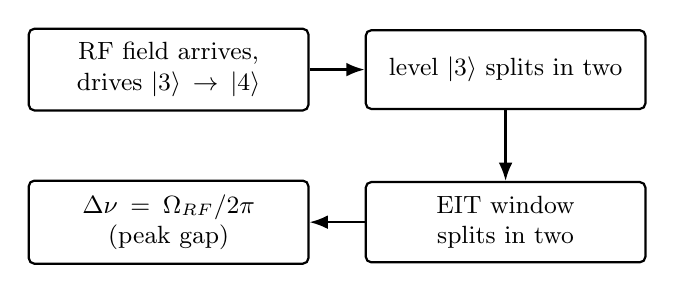
\begin{tikzpicture}
\node[fbox2] (a1) {RF field arrives, drives $\ket3\to\ket4$};
\node[fbox2, right=7mm of a1] (a2) {level $\ket3$ splits in two};
\node[fbox2, below=9mm of a2] (a3) {EIT window splits in two};
\node[fbox2, left=7mm of a3] (a4) {$\Delta\nu=\Omega_{RF}/2\pi$ (peak gap)};
\draw[farr] (a1)--(a2);
\draw[farr] (a2)--(a3);
\draw[farr] (a3)--(a4);
\end{tikzpicture}
\end{center}

\begin{takeaway}
AT splitting is the physical mechanism, EIT is the stage it happens on. Without EIT there is no narrow window to split in the first place; without the RF field there is nothing to split it.
\end{takeaway}

\subsection*{Where does ``communication'' actually enter the physics?}
\begin{itemize}
\item A transmitter (Tx) somewhere far away radiates an RF electric field $E_{RF}$ carrying a data symbol $x$.
\item That field travels through free space, loses strength with distance like any radio wave, and arrives at the vapor cell.
\item That arriving field is exactly what drives the $\ket{3}\to\ket{4}$ transition above.
\item So the ``antenna input'' of this whole system is nothing more exotic than: the RF field's magnitude and phase, physically present at the atoms' location. Everything from here onward --- EIT, AT splitting, $P_{out}$, photodetection --- is simply the read-out chain recovering $x$ from that field.
\end{itemize}

\newpage
% ============================================================
\section{Part III --- The Math Chain from Quantum Physics to $P_{out}$ (Eq.~2--7)}
% ============================================================

\begin{center}
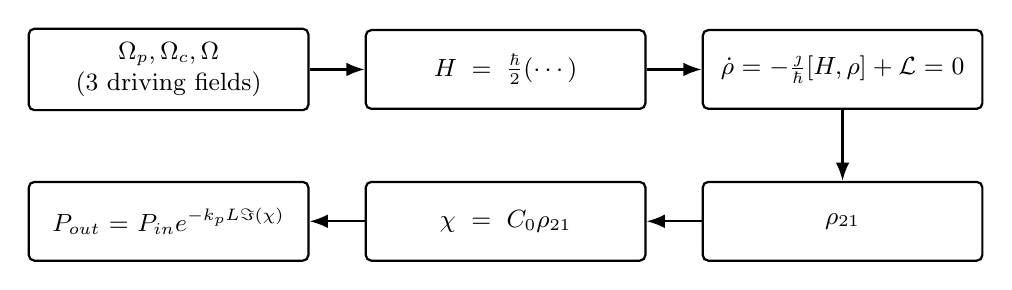
\begin{tikzpicture}
\node[fbox2] (a1) {$\Omega_p,\Omega_c,\Omega$\\(3 driving fields)};
\node[fbox2, right=7mm of a1] (a2) {$H=\frac{\hbar}{2}(\cdots)$};
\node[fbox2, right=7mm of a2] (a3) {$\dot\rho=-\frac{\jmath}{\hbar}[H,\rho]+\mathcal L=0$};
\node[fbox2, below=9mm of a3] (a4) {$\rho_{21}$};
\node[fbox2, left=7mm of a4] (a5) {$\chi=C_0\rho_{21}$};
\node[fbox2, left=7mm of a5] (a6) {$P_{out}=P_{in}e^{-k_pL\Im(\chi)}$};
\draw[farr] (a1)--(a2);
\draw[farr] (a2)--(a3);
\draw[farr] (a3)--(a4);
\draw[farr] (a4)--(a5);
\draw[farr] (a5)--(a6);
\end{tikzpicture}
\end{center}

\subsection*{What does Eq.~(2) actually say?}
\[
P_{out}(t) = P_{in}\exp\{-k_pL\,\Im(\chi(t))\}
\]
\begin{itemize}
\item $P_{in}$: probe laser power going into the cell.
\item $k_p=2\pi/\lambda_p$: the probe laser's wavenumber, how tightly its wave oscillates in space.
\item $L$: the length of the vapor cell --- how much material the light has to travel through.
\item $\Im(\chi(t))$: the absorptive part of susceptibility, time-dependent because it depends on the atoms' quantum state, which depends on the RF field.
\end{itemize}
\begin{eqmeaning}
This is Beer's law of absorption in atomic-physics notation: light going into an absorbing slab comes out weaker, exponentially, the amount of weakening set by how absorbing the material is and how far the light travels through it. If $\Im(\chi)$ swings up and down over time, $P_{out}(t)$ swings too --- this is literally how information gets encoded onto the light.
\end{eqmeaning}
\begin{simuse}
This is the last physics step before anything touches electronics. In every figure's simulation pipeline (Fig.~3 through Fig.~9), $P_{out}$ is computed by plugging the QuTiP-solved $\rho_{21}$ into exactly this formula --- it is never re-derived per figure, only re-evaluated at different $(\Delta_c,\Omega_{RF})$ or $(\Omega_{LO},\Omega_{RF},t)$ points.
\end{simuse}

\subsection*{What does Eq.~(3) actually say?}
\[
P_{in} = \frac{\pi}{2\eta_0}\left(\frac{d\,\Omega_p\hbar}{2\sqrt{\wp_{12}}}\right)^2
\]
\begin{itemize}
\item $\eta_0$: impedance of free space (377\,$\Omega$), converts field-squared into a power.
\item $d$: the $1/e^2$ diameter of the probe laser beam --- how ``fat'' the laser spot is.
\item $\Omega_p$: probe Rabi frequency (what strength of atom-driving you're aiming for).
\item $\wp_{12}$: dipole moment of the $\ket1\to\ket2$ transition, given in the paper's table pre-squared as $(2.5ea_0)^2$, so $\sqrt{\wp_{12}}=2.5ea_0$ is what actually appears in the formula.
\end{itemize}
\begin{eqmeaning}
This equation runs backward from what you might expect: instead of computing $\Omega_p$ from a known laser power, it computes ``how much raw laser power do I need to send in'' given the Rabi frequency you \emph{want} the probe to achieve. It is a design/calibration formula.
\end{eqmeaning}

\subsection*{What does Eq.~(4) actually say?}
\[
\chi(t) = C_0\,\rho_{21}(t), \qquad C_0 = \frac{-2N_0\wp_{12}}{\epsilon_0\hbar\Omega_p}
\]
\begin{itemize}
\item $N_0$: atomic density --- how many atoms per cubic metre are in the cell.
\item $\epsilon_0$: vacuum permittivity, a fixed constant of nature.
\item $C_0$: bundles together everything about the cell that is fixed/unchanging.
\item $\rho_{21}(t)$: the only time-varying piece --- this is where all the RF-field information lives.
\end{itemize}
\begin{eqmeaning}
This is the direct bridge between the abstract quantum number $\rho_{21}$ and the real, physically measurable susceptibility $\chi$. Everything the atoms ``know'' about the RF field lives inside $\rho_{21}$; this equation is how that knowledge becomes an optical property you can shine light through and read.
\end{eqmeaning}

\subsection*{What does the master equation, Eq.~(5), actually say?}
\[
\dot\rho = \frac{\partial\rho}{\partial t} = -\frac{\jmath}{\hbar}[H,\rho] + \mathcal{L}
\]
\begin{itemize}
\item $[H,\rho]$ (the commutator with the Hamiltonian): the clean, reversible, laser-driven part of the evolution --- the ``swinging on a swing'' part.
\item $\mathcal{L}$ (the Lindblad/decay term): the messy, irreversible part --- atoms randomly falling back down and losing their neat quantum coherence.
\end{itemize}
\begin{eqmeaning}
Real atoms always have both effects fighting each other: driven oscillation trying to build up coherence, and decay constantly tearing it back down. The steady-state answer (setting $\dot\rho=0$) is where these two effects balance --- and that balance point is the single number, $\rho_{21}$, that this whole paper is built on extracting.
\end{eqmeaning}
\begin{simuse}
QuTiP does not need you to solve this equation by hand --- you hand it the Hamiltonian matrix (next) and the decay operators, and it numerically finds the steady state $\dot\rho=0$ for you. That numerical solve, repeated over a grid of $(\Delta_c,\Omega_{RF})$, is literally what produces Fig.~3's whole surface.
\end{simuse}

\subsection*{What does the Hamiltonian, Eq.~(6), actually say?}
\[
H = \frac{\hbar}{2}
\begin{pmatrix}
0 & \Omega_p & 0 & 0\\
\Omega_p & -2\Delta_p & \Omega_c & 0\\
0 & \Omega_c & -2(\Delta_p+\Delta_c) & \Omega\\
0 & 0 & \Omega & -2(\Delta_p+\Delta_c+\Delta_{RF})
\end{pmatrix}
\]
\begin{itemize}
\item Off-diagonal entries ($\Omega_p,\Omega_c,\Omega$): the ``connections'' between adjacent levels --- how strongly each laser/field couples that pair together, forming a ladder: 1--2 via probe, 2--3 via coupling, 3--4 via RF/LO.
\item Diagonal entries: detunings --- how far off-resonance each level sits, stacked cumulatively down the ladder.
\item $\Omega$ here is the RF-driven term specifically, and it takes a \emph{different exact form} for the LO-free vs.\ LO-dressed receiver (Parts IV/V) --- this is the one entry that changes between the two receiver designs; everything else in this matrix is shared.
\end{itemize}
\begin{simuse}
This 4$\times$4 matrix, plus the decay operators below, is literally everything you type into QuTiP's \texttt{Qobj}/\texttt{steadystate} call. There is no other hidden physics --- Fig.~3's entire 3D surface is nothing more than solving this exact matrix equation once per grid point.
\end{simuse}

\subsection*{What does the decay (Lindblad) term, Eq.~(7), actually say?}
\[
\mathcal{L} =
\begin{pmatrix}
\gamma_2\rho_{22} & -\gamma_{12}\rho_{12} & -\gamma_{13}\rho_{13} & -\gamma_{14}\rho_{14}\\
-\gamma_{21}\rho_{21} & \gamma_3\rho_{33}-\gamma_2\rho_{22} & -\gamma_{23}\rho_{23} & -\gamma_{24}\rho_{24}\\
-\gamma_{31}\rho_{31} & -\gamma_{32}\rho_{32} & \gamma_4\rho_{44}-\gamma_3\rho_{33} & -\gamma_{34}\rho_{34}\\
-\gamma_{41}\rho_{41} & -\gamma_{42}\rho_{42} & -\gamma_{42}\rho_{42} & -\gamma_4\rho_{44}
\end{pmatrix}, \quad \gamma_{ij}=\frac{\gamma_i+\gamma_j}{2}
\]
\begin{itemize}
\item $\gamma_i$: the spontaneous-decay rate of level $i$ --- how fast that level ``leaks'' population back down.
\item $\gamma_{ij}$: the \emph{coherence} decay rate between levels $i,j$ --- how fast the off-diagonal ``cooperation'' terms get scrambled, simply the average of the two levels' own decay rates.
\end{itemize}
\begin{ifnot}
If $\mathcal{L}$ were zero (no decay at all), the atoms would oscillate forever with no steady state --- $\rho_{21}$ would never settle to a fixed, readable value, and $P_{out}$ would never stabilize into something you could measure.
\end{ifnot}

\subsection{Appendix A --- the analytical steady-state solution (Eq.~39--48)}
QuTiP solves the master equation numerically, but the supplementary material also derives a hand-solvable approximate formula, useful for building intuition and for sanity-checking the numerics.

\subsubsection*{Setting up the chain of equations}
Starting from the commutator expansion
\[
[H,\rho]_{21} = \frac{\hbar\Omega_p}{2}(\rho_{11}-\rho_{22}) - \hbar\Delta_p\rho_{21} + \frac{\hbar\Omega_c}{2}\rho_{31}
\]
one writes the coupled steady-state equations for $\rho_{21},\rho_{31},\rho_{41}$ (Eqs.~40--41b). These three equations are coupled --- $\rho_{21}$ depends on $\rho_{31}$, which depends on $\rho_{41}$ --- so they must be solved together, not one at a time.

\subsubsection*{What assumptions let us solve it by hand?}
\begin{itemize}
\item $\rho_{11}\approx1$, all other diagonal populations $\approx0$: almost every atom sits in the ground state, since the driving fields here are weak compared to what would be needed to noticeably empty it out.
\item $\rho_{32},\rho_{42}\to0$: the ``far'' coherences (between non-adjacent levels in the ladder) are assumed negligible --- their effect on $\rho_{21}$ is a small, second-order correction.
\end{itemize}
\begin{ifnot}
Without these assumptions you would need the full numerical solve every time --- these two simplifications are exactly what makes an algebraic, closed-form answer possible at all.
\end{ifnot}

\subsubsection*{The resulting closed form (Eq.~45)}
\[
\rho_{21} = \dfrac{-\jmath\frac{\Omega_p}{2}}{\gamma_{21}-\jmath\Delta_p-\dfrac{(\Omega_c/2)^2}{\gamma_{31}-\jmath(\Delta_p+\Delta_c)-\dfrac{(\Omega_{RF}/2)^2}{\gamma_{41}-\jmath(\Delta_p+\Delta_c+\Delta_{RF})}}}
\]
\begin{eqmeaning}
This is a ``continued fraction'' --- each level's effect on $\rho_{21}$ is folded in one layer at a time, like nested parentheses. Physically: the probe transition's response is modified by the coupling transition, which is itself modified by the RF transition, cascading down the ladder from level 4 back up to level 1.
\end{eqmeaning}

\subsubsection*{The on-resonance simplification (Eq.~46) and where the two peaks come from (Eq.~48)}
On resonance ($\Delta_p=\Delta_{RF}=0$, $\gamma_{31}=\gamma_{41}=0$):
\[
\Im(\rho_{21}) = \frac{-\Omega_p\gamma_{21}}{\dfrac{\Omega_c^4}{8\left(\dfrac{\Omega_{RF}^2}{4\Delta_c}+\Delta_c\right)^2 + 2\gamma_{21}^2}}
\]
Differentiating with respect to $\Delta_c$ and setting the result to zero gives exactly three turning points:
\[
\Delta_{c,1}=0,\qquad \Delta_{c,2}=\frac{\Omega_{RF}}{2},\qquad \Delta_{c,3}=-\frac{\Omega_{RF}}{2}
\]
\begin{eqmeaning}
This is the algebraic proof --- not just something QuTiP happens to draw --- that the two AT-split peaks sit exactly $\Omega_{RF}$ apart on the $\Delta_c$ axis. This single result is the mathematical backbone underneath both Fig.~3 and Fig.~4.
\end{eqmeaning}
\begin{takeaway}
Appendix A shows, by hand, exactly what QuTiP shows numerically: a weak RF field produces two narrow transparency peaks separated by precisely $\Omega_{RF}$. QuTiP is used because this exact algebra only works cleanly \emph{with} the simplifying assumptions above --- once you drop them (e.g.\ include the LO, Part V), the algebra gets too messy and only survives as an approximation.
\end{takeaway}

\newpage
% ============================================================
\section{Part IV --- The LO-Free Receiver: From RF Field to Bits (Eq.~8--22)}
% ============================================================

\begin{center}
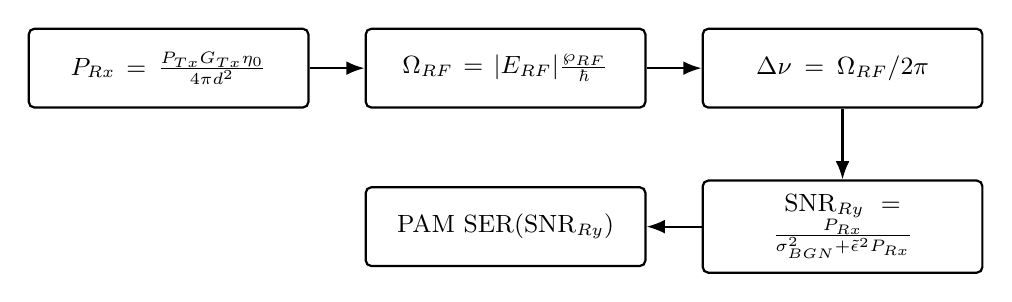
\begin{tikzpicture}
\node[fbox2] (a1) {$P_{Rx}=\frac{P_{Tx}G_{Tx}\eta_0}{4\pi d^2}$};
\node[fbox2, right=7mm of a1] (a2) {$\Omega_{RF}=|E_{RF}|\frac{\wp_{RF}}{\hbar}$};
\node[fbox2, right=7mm of a2] (a3) {$\Delta\nu=\Omega_{RF}/2\pi$};
\node[fbox2, below=9mm of a3] (a4) {$\text{SNR}_{Ry}=\frac{P_{Rx}}{\sigma_{BGN}^2+\tilde\epsilon^2P_{Rx}}$};
\node[fbox2, left=7mm of a4] (a5) {PAM SER$(\text{SNR}_{Ry})$};
\draw[farr] (a1)--(a2);
\draw[farr] (a2)--(a3);
\draw[farr] (a3)--(a4);
\draw[farr] (a4)--(a5);
\end{tikzpicture}
\end{center}

\subsection*{What does Eq.~(8) actually say?}
\[
\Omega_{RF} = |E_{RF}|\,\frac{\wp_{RF}}{\hbar}
\]
\begin{eqmeaning}
The RF Rabi frequency you measure optically (via the AT-splitting gap) is directly proportional to the real RF field strength $|E_{RF}|$ hitting the cell. Since $\Omega_{RF}$ is read straight off the optical spectrum, and this equation relates it linearly to the field, you've turned an electric-field measurement into an optical-frequency measurement --- no electronics touch the RF field itself.
\end{eqmeaning}

\subsection*{What do Eq.~(9) and Eq.~(10) actually say?}
\[
y = \sqrt{P_{Rx}}\,hx + n_{BGN}, \qquad P_{Rx}=\frac{P_{Tx}G_{Tx}}{4\pi d_{Tx\text{-}Rx}^2}\eta_0
\]
\begin{itemize}
\item $x$: the transmitted data symbol (unit-power, random).
\item $h$: the wireless channel, models random fading.
\item $P_{Rx}=|E_{RF}|^2$: received power.
\item $P_{Tx}$, $G_{Tx}$, $d_{Tx\text{-}Rx}$: transmit power, transmit antenna gain, distance.
\end{itemize}
\begin{eqmeaning}
Eq.~(10) is the ordinary inverse-square-law free-space path loss any radio link obeys --- nothing atomic-physics-specific yet. This is exactly where the ``communications'' half of the paper begins: everything before this point was pure atomic physics (how the field gets read optically); everything from here on is standard wireless-systems bookkeeping built on top of that atomic readout.
\end{eqmeaning}

\subsection*{What does Eq.~(11) actually say?}
\[
z = \frac{\wp_{RF}}{\hbar}\left|\sqrt{P_{Rx}}\,hx+n_{Ry}\right|
\]
\begin{eqmeaning}
This combines Eq.~(8)'s readout relationship with the wireless channel of Eq.~(9): $z$ is literally what a lock-in amplifier reads off the AT-splitting measurement, with noise $n_{Ry}$ mixed in. The absolute-value bars are the important detail: \textbf{the LO-free receiver can only ever measure a magnitude} (a splitting gap is always positive) --- it structurally cannot see the sign or phase of $x$. This one detail is the root cause of everything that makes LO-free receivers ``amplitude-only.''
\end{eqmeaning}

\subsection*{What are the three noise sources, Eq.~(12)--(14)?}
\begin{itemize}
\item \textbf{Quantum projection noise (QPN)}, Eq.~(12): $\sigma_{QPN}^2\approx \dfrac{1}{4C_{eff}N_{atoms}}$. A fundamental quantum-measurement limit --- even a perfect experiment has randomness from measuring a finite number of atoms $N_{atoms}$, tempered by readout efficiency $C_{eff}\le1$. With very large $N_{atoms}$ this becomes tiny and is neglected throughout.
\item \textbf{Thermal noise}, Eq.~(13): $\sigma_{TN}^2=4k_BTB$. Ordinary Johnson-Nyquist electrical noise from the classical electronics, proportional to temperature $T$ and bandwidth $B$.
\item \textbf{Observation uncertainty}, Eq.~(14): $\sigma_{UN}^2=(\tilde\epsilon E_{RF})^2$. When $\Omega_{RF}$ gets small, the two AT peaks start to blur together and become harder to pinpoint precisely; this term captures that measurement blur, scaled by a fixed fractional uncertainty $\tilde\epsilon=0.5\%$ (paper-stated, sourced from Sedlacek et al.\ 2012).
\end{itemize}
\begin{ifnot}
Without $\sigma_{UN}^2$ specifically, the model would predict perfect readout accuracy no matter how weak $\Omega_{RF}$ got, which is unphysical --- a vanishingly small AT-splitting gap genuinely cannot be measured with infinite precision by any real instrument.
\end{ifnot}

\subsection*{What do Eq.~(15) and Eq.~(16) actually say?}
\[
\sigma_{Ry}^2=\sigma_{UN}^2+\sigma_{QPN}^2+\sigma_{BGN}^2, \qquad
\text{SNR}_{Ry}=\frac{P_{Rx}|h|^2}{\sigma_{BGN}^2+\sigma_{QPN}^2+\tilde\epsilon^2 P_{Rx}}
\]
\begin{eqmeaning}
Look carefully at the denominator: it has a \emph{fixed} noise floor ($\sigma_{BGN}^2$) plus a term that grows \emph{with the signal itself} ($\tilde\epsilon^2P_{Rx}$). This is unusual --- in a normal radio, more received power always means a better SNR without limit. Here, because $\tilde\epsilon$ scales with the field strength, pushing $P_{Rx}$ to infinity makes SNR approach a hard ceiling $1/\tilde\epsilon^2$ instead of growing forever. This is a real, algebraically provable property of this exact equation, not a coding mistake --- and it has been checked and re-checked extensively against this equation on its own terms.
\end{eqmeaning}
\begin{simuse}
Because of this ceiling, LO-free curves in every SNR-domain figure (Fig.~7, 8, 9c) can only ever occupy a narrow SNR band near $1/\tilde\epsilon^2$ before the formula itself becomes meaningless. Any LO-free simulation needs to check this ceiling first, or the resulting curve will silently make no physical sense at high SNR.
\end{simuse}

\subsection*{How does the mutual-information chain, Eq.~(17)--(22), actually work?}
The paper wants to know: given the noisy observation $z$, how many bits per channel use can actually be reliably communicated? This needs \emph{mutual information} $I(z;x)=H(z)-H(z|x)$ (Eq.~17) --- ``how much does knowing $z$ reduce your uncertainty about $x$.''
\begin{itemize}
\item Because $z$ is a noisy magnitude-only reading (Eq.~11's absolute value), it follows a \textbf{Rayleigh distribution} (Eq.~19) with no signal present, and a \textbf{Rician distribution} once a signal $x$ is added --- the standard statistical distributions for ``the magnitude of a noisy 2D vector.''
\item $H(z)$, the marginal entropy (Eq.~20), measures the raw randomness of the observation before you know $x$.
\item $H(z|x)$, the conditional entropy (Eq.~21), measures the leftover randomness once $x$ is already known; it involves modified Bessel functions $I_0,I_1$, the standard machinery for Rician statistics.
\item Combining them, Eq.~(22):
\[
\mathcal{I}(z;x)=\frac12\ln\!\left(\frac{\pi(\mathfrak r+1)}{2}\right) - \ln I_0(\mathfrak r) + \mathfrak r\frac{I_1(\mathfrak r)}{I_0(\mathfrak r)}, \qquad \mathfrak r\approx \text{SNR}_{Ry}
\]
\end{itemize}
\begin{plain}
You don't need to re-derive this to use it --- just know it is the ``exchange rate'' between SNR and usable bits/second/Hz, specifically for a receiver that can only measure amplitude, not phase. It always gives fewer bits, at the same SNR, than an ideal receiver that could see both amplitude and phase (Part V, next).
\end{plain}
\begin{takeaway}
The LO-free receiver's whole story, top to bottom: measure a field's magnitude via an optical peak-gap $\to$ that magnitude is degraded both by ordinary noise and by its own measurement-uncertainty $\to$ that combined effect caps SNR at $1/\tilde\epsilon^2$ $\to$ feed that SNR into a Rician (not Gaussian) mutual-information formula, because you only ever saw a magnitude, never a phase.
\end{takeaway}

\newpage
% ============================================================
\section{Part V --- The LO-Dressed Receiver: The Atomic Mixer (Eq.~23--38)}
% ============================================================

\begin{center}
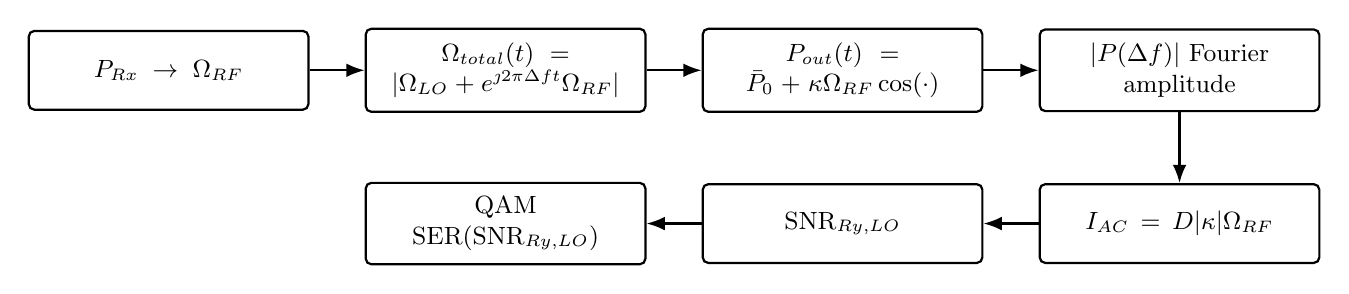
\begin{tikzpicture}
\node[fbox2] (a1) {$P_{Rx}\to\Omega_{RF}$};
\node[fbox2, right=7mm of a1] (a2) {$\Omega_{total}(t)=|\Omega_{LO}+e^{\jmath2\pi\Delta ft}\Omega_{RF}|$};
\node[fbox2, right=7mm of a2] (a3) {$P_{out}(t)=\bar P_0+\kappa\Omega_{RF}\cos(\cdot)$};
\node[fbox2, right=7mm of a3] (a4) {$|P(\Delta f)|$ Fourier amplitude};
\node[fbox2, below=9mm of a4] (a5) {$I_{AC}=D|\kappa|\Omega_{RF}$};
\node[fbox2, left=7mm of a5] (a6) {$\text{SNR}_{Ry,LO}$};
\node[fbox2, left=7mm of a6] (a7) {QAM SER$(\text{SNR}_{Ry,LO})$};
\draw[farr] (a1)--(a2);
\draw[farr] (a2)--(a3);
\draw[farr] (a3)--(a4);
\draw[farr] (a4)--(a5);
\draw[farr] (a5)--(a6);
\draw[farr] (a6)--(a7);
\end{tikzpicture}
\end{center}

\subsection*{What do Eq.~(23)--(25) actually say?}
The LO-dressed receiver adds a second, always-on RF-like field called the \textbf{local oscillator (LO)}, on resonance with the same $\ket3\to\ket4$ transition. The RF signal and LO add together as ordinary waves:
\[
E_{total}=E_{LO}+E_{RF} = \sqrt{A_{LO}^2+A_{RF}^2+2A_{LO}A_{RF}\cos(2\pi\Delta f\,t+\Delta\phi)}\;\cos(2\pi f_{LO}t+\phi_{LO})
\]
\begin{plain}
Two tones close together in frequency ``beat'' against each other, producing a slow envelope that rises and falls at the \emph{difference} frequency $\Delta f=f_{LO}-f_{RF}$. This is exactly how an old-fashioned superheterodyne radio mixer works, done here with atoms instead of a diode.
\end{plain}
Since $A_{RF}\ll A_{LO}$ (the LO is deliberately much stronger), a Taylor expansion (Eq.~25) simplifies this to
\[
E_{total}\approx[A_{LO}+A_{RF}\cos(2\pi\Delta f\,t+\Delta\phi)]\cos(2\pi f_{LO}t+\phi_{LO})
\]
\begin{eqmeaning}
The fast LO carrier ($\cos(2\pi f_{LO}t)$, which sets up the AT splitting) has its amplitude slowly modulated by exactly the weak RF signal's beat note. Both the RF signal's amplitude \emph{and} phase survive, riding on top of the LO's carrier, at the slow, easy-to-measure beat frequency $\Delta f$ (150\,kHz here) instead of at the RF carrier's own frequency (3.5\,GHz). This is the whole trick that lets the LO-dressed receiver recover phase, which the LO-free receiver structurally cannot (compare to Eq.~11's absolute-value bars).
\end{eqmeaning}

\subsection*{What does Eq.~(26) actually say?}
\[
\rho_{21}\big|_{\Delta_p=\Delta_c=\Delta_{LO}=0,\gamma_3=\gamma_4=0} = \frac{\jmath\gamma_2\Omega_p|\Omega_{total}|^2}{\gamma_2^2|\Omega_{total}|^2+2\Omega_p^2(\Omega_c^2+\Omega_p^2+|\Omega_{total}|^2)}, \quad \Omega_{total}=\left|\Omega_{LO}+e^{\jmath(2\pi\Delta ft+\Delta\phi)}\Omega_{RF}\right|
\]
\begin{itemize}
\item Two simplifications make this tractable: (1) every field is exactly on resonance ($\Delta_p=\Delta_c=\Delta_{LO}=0$), and (2) the two Rydberg levels are treated as effectively non-decaying ($\gamma_3\approx\gamma_4\approx0$), since their real lifetimes are so much longer than $\gamma_2$'s that they barely matter here.
\item $\Omega_{total}$ plays exactly the same slot in the Hamiltonian that plain $\Omega_{RF}$ played in Eq.~(6) for the LO-free case --- this is why Fig.~5's static curve can literally reuse Fig.~3's own computed data, just relabeled.
\end{itemize}

\subsection*{What does Eq.~(27) actually say?}
\[
P_{out}(t) \approx \bar P_0 + \kappa\Omega_{RF}\cos(2\pi\Delta f\,t+\Delta\phi)
\]
\begin{eqmeaning}
This is the single most important equation for the LO-dressed receiver: the probe transmission is a DC baseline $\bar P_0$ (set almost entirely by the LO, since the RF signal is comparatively tiny) plus a small oscillating term whose \emph{amplitude} is directly proportional to $\Omega_{RF}$, oscillating at the easy-to-measure beat frequency $\Delta f$. Reading off that oscillation's amplitude and phase directly gives back the RF signal's amplitude and phase. $\kappa$ is the ``gain'' of this whole conversion --- microwatts of $P_{out}$ swing per unit of $\Omega_{RF}$ input; it is exactly the slope of the Fig.~5(a) curve at the operating point.
\end{eqmeaning}
\begin{ifnot}
If $\kappa$ were zero (a flat, unresponsive operating point), the receiver would be completely blind: any RF signal would produce zero output swing, no matter how strong. Maximizing $|\kappa|$ is the single design goal for this whole receiver, which is exactly what Appendix B (below) solves for.
\end{ifnot}

\subsection*{What do Eq.~(28) and Eq.~(29) actually say?}
\[
P_{readout}(t)=P_{out}(t)-\bar P_0 = |P(\Delta f)|\cos(2\pi\Delta f\,t+\Delta\phi), \qquad
\Omega_{RF}=\frac{|P(\Delta f)|}{|\kappa|}
\]
\begin{itemize}
\item $|P(\Delta f)|$: the amplitude of the single-sided Fourier spectrum of $P_{out}(t)$, evaluated exactly at the beat frequency $\Delta f$ --- Fourier-transform the measured output waveform, and read off how tall the spike is at $\Delta f$.
\item Dividing that spike height by the known gain $\kappa$ directly gives back $\Omega_{RF}$; the phase of that same Fourier component gives back $\Delta\phi$, hence $\phi_{RF}$.
\end{itemize}
\begin{simuse}
This is the demodulation step --- the atomic-physics equivalent of an FM/AM radio's discriminator circuit. Fig.~5(b) and Fig.~5(c) are exactly Eq.~(24)/(27) plotted out: (b) is the phasor magnitude $|\Omega_{total}(t)|$ feeding in, (c) is the resulting $P_{out}(t)$ coming out.
\end{simuse}

\subsection*{What do Eq.~(30)--(37) actually say --- the full electrical chain?}
\[
z^{LO}=\sqrt{P_{Rx}G_{LNA}R_LD}\,|\kappa|\frac{\wp_{RF}}{\hbar}\,hx+n_{Ry,LO}
\]
This chains together every physical conversion step:
\begin{enumerate}[nosep]
\item RF field $\to$ photocurrent: $I_{AC}=D|\kappa|\Omega_{RF}$, where $D$ is the photodiode's responsivity (amps out per watt of light in).
\item Photocurrent $\to$ electrical power: $P_{eAC}=I_{AC}^2R_L$, ordinary $P=I^2R$ with load resistance $R_L$.
\item Amplification: $P_{LNA}=G_{LNA}P_{eAC}+\sigma_{TN}^2$, with LNA gain $G_{LNA}$.
\end{enumerate}
The noise budget (Eq.~36) has three pieces, added as variances since they are independent random processes:
\begin{itemize}
\item \textbf{Background noise contribution}: the same $\sigma_{BGN}^2$ from before, now passed through the same $\kappa,D,G_{LNA},R_L$ gain chain as the signal itself.
\item \textbf{Photon shot noise}, $\sigma_{PSN}^2=2eB\bar I$ (Eq.~34): unavoidable graininess in a light beam's photon-arrival statistics; $\bar I=\eta_{eff}\frac{|P(\Delta f)|}{\hbar f_p}e$ (Eq.~35) is the average photocurrent, $\eta_{eff}$ the photon-to-electron efficiency.
\item \textbf{Thermal noise}, $\sigma_{TN}^2$: the same Johnson noise as Eq.~(13), from the electronics.
\end{itemize}
Putting it together, Eq.~(37):
\[
\text{SNR}_{Ry,LO}=\frac{G_{LNA}R_LD^2\kappa^2\left(\frac{\wp_{RF}}{\hbar}\right)^2P_{Rx}|h|^2}{\sigma_{Ry,LO}^2}
\]
\begin{eqmeaning}
Compare to Eq.~(16)'s LO-free SNR: here the noise floor $\sigma_{Ry,LO}^2$ does \emph{not} grow with the signal power --- it's essentially fixed (dominated by thermal + shot noise, largely independent of how strong the incoming RF signal is). That is the deep mathematical reason LO-dressed SNR keeps climbing with distance/power far past where LO-free saturates at its $1/\tilde\epsilon^2$ ceiling --- as long as you stay inside the linear region where Eq.~(27) is valid.
\end{eqmeaning}

\subsection*{What does Eq.~(38) actually say?}
\[
\mathcal{I}(z^{LO};x) = e^{1/\text{SNR}_{Ry,LO}}\,E_1(1/\text{SNR}_{Ry,LO})\,\ln 2, \qquad E_1(x)=\int_x^\infty\frac{e^{-t}}{t}\,dt
\]
This is the standard closed-form ergodic (average) channel capacity of a Rayleigh-faded complex Gaussian channel, in bits/s/Hz --- it applies here because, unlike LO-free, the LO-dressed receiver recovers \emph{both} amplitude and phase, so its observation is a full complex-Gaussian-style channel, not a magnitude-only one.
\begin{plain}
$E_1$ (the ``exponential integral'') is a standard tabulated math function, the same way $\sin$ or $\ln$ are --- every numerical library (e.g.\ SciPy's \texttt{scipy.special.exp1}) has it built in.
\end{plain}

\subsection{Appendix B --- $\kappa$, $\Gamma_{EIT}$ versus $\Gamma$, and the optimal LO point (Eq.~49--58)}

\subsubsection*{Difference between $\Gamma_{EIT}$ and $\Gamma$}
\begin{itemize}
\item $\Gamma_{EIT}$ = the natural linewidth of the plain, three-level EIT transparency window (no LO, no RF), derived analytically in Eq.~(51):
\[
\Gamma_{EIT}=\frac{\Omega_c^2+\Omega_p^2}{2\sqrt{\gamma_2^2+2\Omega_p^2}}
\]
It depends only on the probe Rabi frequency $\Omega_p$, coupling Rabi frequency $\Omega_c$, and the decoherence rate $\gamma_2$. Physically: it sets how wide the plain transparency window is.
\item $\Gamma$ = the effective half-width at half-maximum (HWHM) of the full four-level system, once the LO is included:
\[
\Gamma = \Omega_p\sqrt{2(\Omega_c^2+\Omega_p^2)}\Big/2\sqrt{\Omega_p^2+\gamma_2^2}, \qquad \Gamma = \frac{2\sqrt2\,\Omega_p}{\sqrt{\Omega_c^2+\Omega_p^2}}\Gamma_{EIT}
\]
It's related to $\Gamma_{EIT}$ but adjusted for the extra dynamics the LO introduces. Physically: it's the broadened linewidth that sets the sensitivity range of the LO-dressed receiver specifically.
\end{itemize}
\begin{takeaway}
$\Gamma_{EIT}$ = the ``pure'' three-level transparency width. $\Gamma$ = the ``practical'' width once LO mixing is included. Every LO-dressed formula from here on uses $\Gamma$, not $\Gamma_{EIT}$.
\end{takeaway}

\subsubsection*{What does Eq.~(49) actually say?}
\[
\Im[\rho_{21}(\Omega_{RF})]=\bar A\big[1-\Lambda(\Omega_{LO},\Gamma) - \kappa_\rho\Omega_{RF}\cos(2\pi\Delta f\,t+\Delta\phi)\big]
\]
\begin{itemize}
\item $\bar A=\gamma_2\Omega_p/(\gamma_2^2+2\Omega_p^2)$: baseline amplitude of probe absorption --- the overall height of the plain 3-level EIT spectrum.
\item $\Lambda(\Omega_{LO},\Gamma)$: the Lorentzian term --- how the LO's own Rabi frequency sets the shape/position of the transparency window it sits on.
\item $\kappa_\rho=\partial\Lambda(\Omega_{LO},\Gamma)/\partial\Omega_{LO}$: the slope (gain coefficient) --- sensitivity to RF changes, i.e.\ how much absorption changes per unit change in $\Omega_{RF}$.
\item $\Omega_{RF}\cos(\dots)$: the actual RF signal, amplitude and phase together.
\end{itemize}
\begin{eqmeaning}
Meaning: probe absorption equals a fixed baseline, minus how much the LO has already suppressed it (the Lorentzian term), minus the small extra wiggle caused by the RF signal riding on top. Everything the receiver ultimately measures is that last, small wiggle term.
\end{eqmeaning}

\subsubsection*{What does Eq.~(51) actually say? (repeated here in its LO-dressed context)}
\[
\Gamma_{EIT}=\frac{\Omega_c^2+\Omega_p^2}{2\sqrt{\gamma_2^2+2\Omega_p^2}}
\]
Meaning: stronger lasers (bigger $\Omega_c,\Omega_p$) broaden the transparency window; more decoherence ($\gamma_2$) narrows it. This defines the natural linewidth the whole LO-dressed sensitivity calculation is built around.

\subsubsection*{What does Eq.~(54) actually say --- the optimal LO strength}
You want the steepest possible slope $|\kappa_\rho|$ --- i.e.\ set the Lorentzian's second derivative to zero (Eq.~53). Solving gives one physically meaningful answer:
\[
\Omega_{LO}=\frac{\sqrt3}{3}\Gamma \quad\Rightarrow\quad (\kappa_\rho)_{max}=\frac{3\sqrt3}{8\Gamma}
\]
\begin{plain}
Think of the Lorentzian bump as a hill. The very steepest point on a bell-curve-shaped hill isn't at the summit (slope $=0$ there) and isn't way out on the flat tail either (slope $\approx0$ there too) --- it's at a specific point partway down the side. This is calculus finding exactly that steepest point, in units of the linewidth $\Gamma$.
\end{plain}
\begin{eqmeaning}
Meaning: this tells you exactly how strong the LO must be set to bias the atoms into their most responsive regime --- park $\Omega_{LO}$ anywhere else and you get a smaller signal for the same $\Omega_{RF}$, i.e.\ a worse receiver.
\end{eqmeaning}
Carrying this through the full, non-simplified $P_{out}$ expression (accounting for $\bar P_0$ itself also depending on $\Omega_{LO}$) shifts the true optimum slightly, Eq.~(58):
\[
\Omega_{LO} = \sqrt{\bar A - 1+\sqrt{\bar A^2-2\bar A+4}}\;\frac{\sqrt3}{3}\Gamma
\]
This is exactly the $(\Omega_{LO})_{opt}$ callout marked on Fig.~5(a).

\subsubsection*{What does Eq.~(56) actually say?}
\[
P_{out}(t) \approx \bar P_0 + \kappa\,\bar P_0\,\Omega_{RF}\cos(2\pi\Delta f\,t+\Delta\phi)
\]
\begin{itemize}
\item $\bar P_0$: baseline probe transmission.
\item $\kappa$: gain coefficient (sensitivity).
\end{itemize}
Meaning: probe transmission equals baseline plus RF modulation. This is exactly the signal the photodetector physically sees, and it is the same equation as Eq.~(27), written out with $\bar P_0$'s own dependence made explicit.

\begin{simuse}
Appendix B's equations give closed-form formulas for baseline, linewidth, and sensitivity. In simulation, you can: set the LO strength using Eq.~(54)/(58); define the transparency window's width using $\Gamma$ and $\Gamma_{EIT}$; calculate probe transmission versus RF signal using Eq.~(56)/(27). This is exactly how the paper generates its SNR curves, linear-dynamic-range plots, and distortion regions without re-solving the full master equation from scratch every single time --- and the formulas are cross-checked against real QuTiP simulations to confirm they stay physically consistent.
\end{simuse}

\begin{takeaway}
Transparency window = the frequency range where probe light passes through the atoms. $\Gamma_{EIT}$ = natural linewidth of that window with no LO; $\Gamma$ = effective linewidth once LO mixing is included. Appendix B's equations are the bridge between raw quantum theory and the usable, closed-form SNR/capacity/SER results shown later in the paper.
\end{takeaway}

\newpage
% ============================================================
\section{Part VI --- The Complete Mental Model}
% ============================================================
Putting every chain from Parts III--V side by side:

\textbf{Atomic physics layer:}
\begin{center}
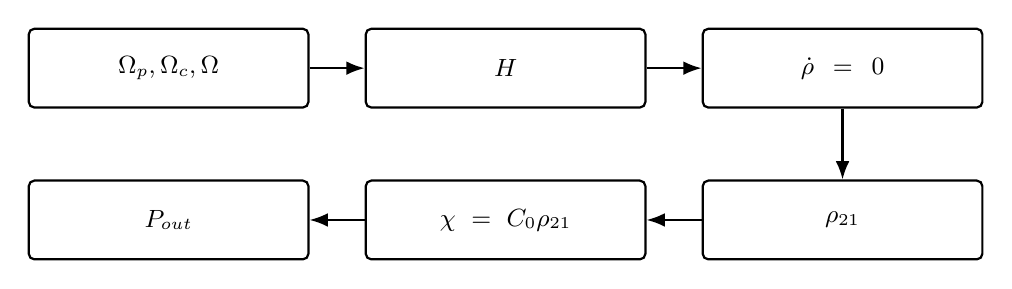
\begin{tikzpicture}
\node[fbox2] (a1) {$\Omega_p,\Omega_c,\Omega$};
\node[fbox2, right=7mm of a1] (a2) {$H$};
\node[fbox2, right=7mm of a2] (a3) {$\dot\rho=0$};
\node[fbox2, below=9mm of a3] (a4) {$\rho_{21}$};
\node[fbox2, left=7mm of a4] (a5) {$\chi=C_0\rho_{21}$};
\node[fbox2, left=7mm of a5] (a6) {$P_{out}$};
\draw[farr] (a1)--(a2); \draw[farr] (a2)--(a3); \draw[farr] (a3)--(a4);
\draw[farr] (a4)--(a5); \draw[farr] (a5)--(a6);
\end{tikzpicture}
\end{center}

\textbf{LO-free communication layer:}
\begin{center}
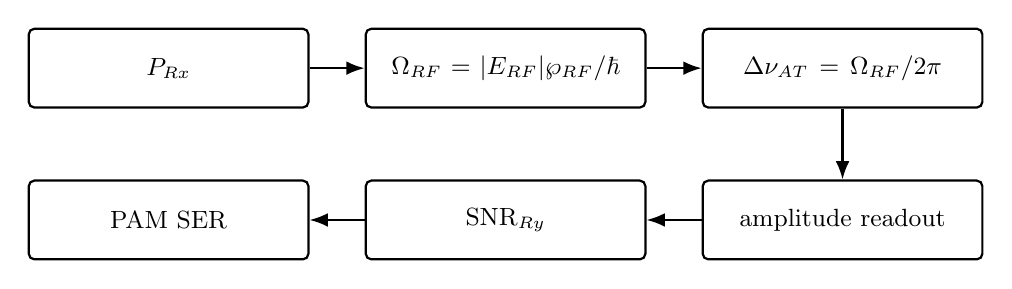
\begin{tikzpicture}
\node[fbox2] (a1) {$P_{Rx}$};
\node[fbox2, right=7mm of a1] (a2) {$\Omega_{RF}=|E_{RF}|\wp_{RF}/\hbar$};
\node[fbox2, right=7mm of a2] (a3) {$\Delta\nu_{AT}=\Omega_{RF}/2\pi$};
\node[fbox2, below=9mm of a3] (a4) {amplitude readout};
\node[fbox2, left=7mm of a4] (a5) {$\text{SNR}_{Ry}$};
\node[fbox2, left=7mm of a5] (a6) {PAM SER};
\draw[farr] (a1)--(a2); \draw[farr] (a2)--(a3); \draw[farr] (a3)--(a4);
\draw[farr] (a4)--(a5); \draw[farr] (a5)--(a6);
\end{tikzpicture}
\end{center}

\textbf{LO-dressed communication layer:}
\begin{center}
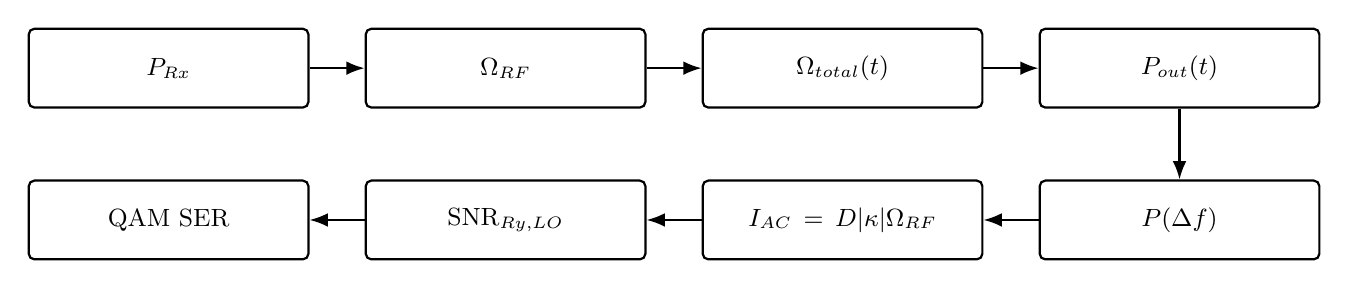
\begin{tikzpicture}
\node[fbox2] (a1) {$P_{Rx}$};
\node[fbox2, right=7mm of a1] (a2) {$\Omega_{RF}$};
\node[fbox2, right=7mm of a2] (a3) {$\Omega_{total}(t)$};
\node[fbox2, right=7mm of a3] (a4) {$P_{out}(t)$};
\node[fbox2, below=9mm of a4] (a5) {$P(\Delta f)$};
\node[fbox2, left=7mm of a5] (a6) {$I_{AC}=D|\kappa|\Omega_{RF}$};
\node[fbox2, left=7mm of a6] (a7) {$\text{SNR}_{Ry,LO}$};
\node[fbox2, left=7mm of a7] (a8) {QAM SER};
\draw[farr] (a1)--(a2); \draw[farr] (a2)--(a3); \draw[farr] (a3)--(a4);
\draw[farr] (a4)--(a5); \draw[farr] (a5)--(a6); \draw[farr] (a6)--(a7); \draw[farr] (a7)--(a8);
\end{tikzpicture}
\end{center}

The distortion mechanisms are opposite, and this is the single most important physical contrast in the whole paper:
\begin{center}
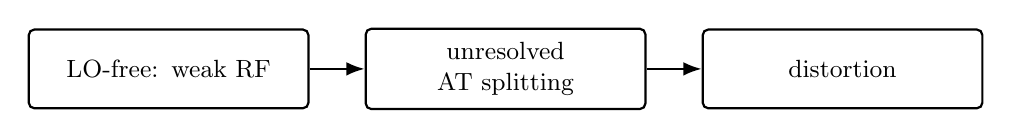
\begin{tikzpicture}
\node[fbox2] (a1) {LO-free: weak RF};
\node[fbox2, right=7mm of a1] (a2) {unresolved AT splitting};
\node[fbox2, right=7mm of a2] (a3) {distortion};
\draw[farr] (a1)--(a2); \draw[farr] (a2)--(a3);
\end{tikzpicture}

\medskip
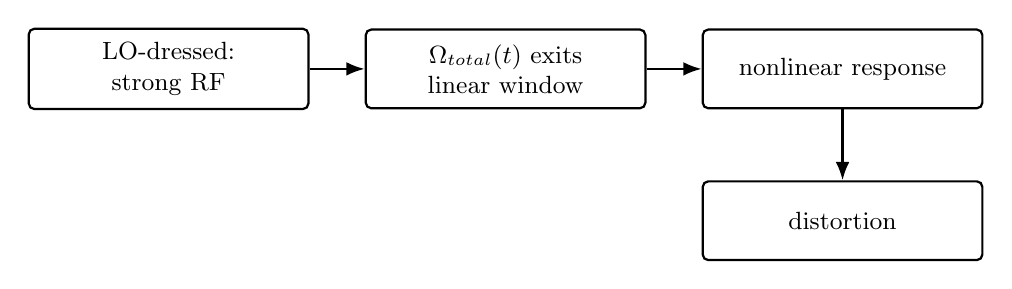
\begin{tikzpicture}
\node[fbox2] (b1) {LO-dressed: strong RF};
\node[fbox2, right=7mm of b1] (b2) {$\Omega_{total}(t)$ exits linear window};
\node[fbox2, right=7mm of b2] (b3) {nonlinear response};
\node[fbox2, below=9mm of b3] (b4) {distortion};
\draw[farr] (b1)--(b2); \draw[farr] (b2)--(b3); \draw[farr] (b3)--(b4);
\end{tikzpicture}
\end{center}

\begin{plain}
LO-free struggles when the signal is too \emph{weak} (the two peaks blur together). LO-dressed struggles when the signal is too \emph{strong} (it overdrives the receiver out of its straight-line region). That is the central physical reason the two Rydberg receiver configurations are complementary: one covers close-in/strong-signal territory, the other covers far-away/weak-signal territory, and between them they cover a much wider range than either could alone.
\end{plain}
\begin{takeaway}
If you remember nothing else from this entire document, remember this: both receivers read out the exact same quantity, $\rho_{21}\to P_{out}$, but they fail in opposite directions, for opposite physical reasons, at opposite ends of the signal-strength scale.
\end{takeaway}

\newpage
% ============================================================
\section{Part VII --- Figure-by-Figure: The Complete Working Math}
% ============================================================
This part writes out the \emph{actual formulas}, in the exact order they are evaluated, for every figure --- not just which paper equation each figure ``uses,'' but the literal computational chain, symbol by symbol, that turns raw parameters into the plotted curve. Every figure after Fig.~3 reuses Fig.~3's underlying quantum-response data rather than re-solving the master equation from scratch --- this is the single most important organizing fact for the whole numerical pipeline.

\begin{center}
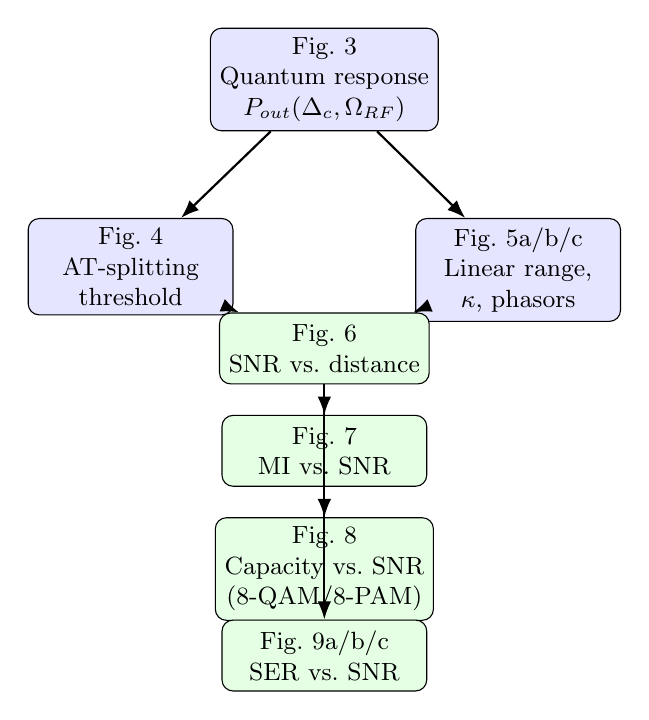
\begin{tikzpicture}[
  box/.style={draw, rounded corners, minimum width=2.6cm, minimum height=0.9cm, align=center, font=\small},
  arr/.style={-{Latex}, thick}
]
\node[box, fill=blue!10] (f3) {Fig.~3\\Quantum response\\$P_{out}(\Delta_c,\Omega_{RF})$};
\node[box, fill=blue!10, below left=1.1cm and -0.3cm of f3] (f4) {Fig.~4\\AT-splitting\\threshold};
\node[box, fill=blue!10, below right=1.1cm and -0.3cm of f3] (f5) {Fig.~5a/b/c\\Linear range,\\$\kappa$, phasors};
\node[box, fill=green!10, below=2.3cm of f3] (f6) {Fig.~6\\SNR vs.\ distance};
\node[box, fill=green!10, below=3.6cm of f3] (f7) {Fig.~7\\MI vs.\ SNR};
\node[box, fill=green!10, below=4.9cm of f3] (f8) {Fig.~8\\Capacity vs.\ SNR\\(8-QAM/8-PAM)};
\node[box, fill=green!10, below=6.2cm of f3] (f9) {Fig.~9a/b/c\\SER vs.\ SNR};
\draw[arr] (f3) -- (f4);
\draw[arr] (f3) -- (f5);
\draw[arr] (f4) -- (f6);
\draw[arr] (f5) -- (f6);
\draw[arr] (f6) -- (f7);
\draw[arr] (f6) -- (f8);
\draw[arr] (f6) -- (f9);
\end{tikzpicture}
\end{center}

\subsection*{Fig.~3 --- $P_{out}(\Delta_c,\Omega_{RF})$}
\textbf{Step 1.} Fix $\Delta_p=0$, $\Delta_{RF}=0$. Sweep a 2D grid of $(\Delta_c,\Omega_{RF})$.
\textbf{Step 2.} At every grid point, build the $4\times4$ Hamiltonian (Eq.~6) with that point's $\Delta_c$ and $\Omega=\Omega_{RF}$, and the fixed decay operators (Eq.~7).
\textbf{Step 3.} Solve $\dot\rho=0$ numerically (QuTiP \texttt{steadystate}) $\Rightarrow$ get $\rho_{21}$ at that point.
\textbf{Step 4.} $\chi = C_0\rho_{21}$ (Eq.~4), then $P_{out}=P_{in}\exp\{-k_pL\,\Im(\chi)\}$ (Eq.~2), with $P_{in}$ fixed once from Eq.~(3).
\[
\boxed{P_{out}(\Delta_c,\Omega_{RF}) = P_{in}\exp\Big\{-k_pLC_0\,\Im\big[\rho_{21}(\Delta_c,\Omega_{RF})\big]\Big\}}
\]
\begin{center}
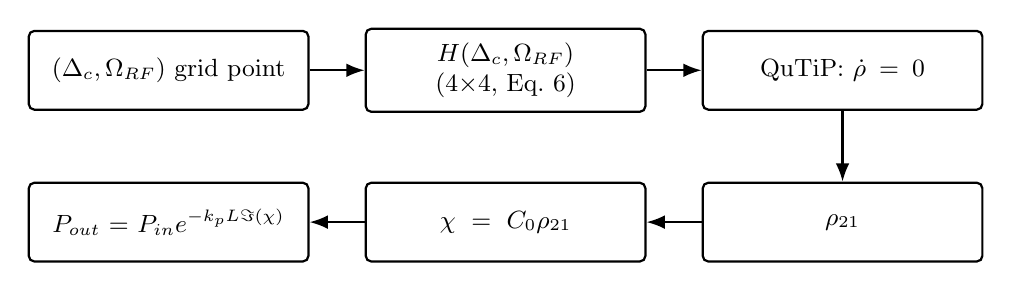
\begin{tikzpicture}
\node[fbox2] (a1) {$(\Delta_c,\Omega_{RF})$ grid point};
\node[fbox2, right=7mm of a1] (a2) {$H(\Delta_c,\Omega_{RF})$ (4$\times$4, Eq.~6)};
\node[fbox2, right=7mm of a2] (a3) {QuTiP: $\dot\rho=0$};
\node[fbox2, below=9mm of a3] (a4) {$\rho_{21}$};
\node[fbox2, left=7mm of a4] (a5) {$\chi=C_0\rho_{21}$};
\node[fbox2, left=7mm of a5] (a6) {$P_{out}=P_{in}e^{-k_pL\Im(\chi)}$};
\draw[farr] (a1)--(a2); \draw[farr] (a2)--(a3); \draw[farr] (a3)--(a4);
\draw[farr] (a4)--(a5); \draw[farr] (a5)--(a6);
\end{tikzpicture}
\end{center}
Repeating Steps~2--4 across the whole grid produces the entire 3D surface --- there is no other formula involved; Fig.~3 IS this loop.

\subsection*{Fig.~4 --- AT-splitting threshold}
\textbf{Step 1.} Reuse Fig.~3's grid, no new solve.
\textbf{Step 2.} Compute the EIT linewidth in closed form (Eq.~51):
\[
\Gamma_{EIT}=\frac{\Omega_c^2+\Omega_p^2}{2\sqrt{\gamma_2^2+2\Omega_p^2}}
\]
\textbf{Step 3.} Define the resolvability criterion: two AT peaks separated by $\Omega_{RF}$ are called resolvable once their separation exceeds twice the HWHM, i.e.\ one full linewidth:
\[
\boxed{\Omega_{RF,th} = 2\,\Gamma_{EIT}}
\]
\begin{eqmeaning}
This is the standard Rayleigh resolution criterion, borrowed from optics: two overlapping peaks are ``just resolved'' once their centers are at least one linewidth apart. Below that separation, the two peaks blur into a single bump on the $P_{out}$ vs.\ $\Delta_c$ curve, and reading off a splitting gap becomes meaningless.
\end{eqmeaning}
\begin{center}
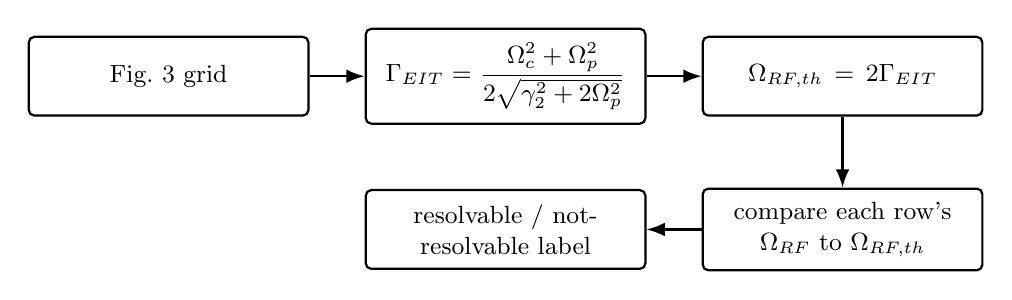
\begin{tikzpicture}
\node[fbox2] (a1) {Fig.~3 grid};
\node[fbox2, right=7mm of a1] (a2) {$\Gamma_{EIT}=\dfrac{\Omega_c^2+\Omega_p^2}{2\sqrt{\gamma_2^2+2\Omega_p^2}}$};
\node[fbox2, right=7mm of a2] (a3) {$\Omega_{RF,th}=2\Gamma_{EIT}$};
\node[fbox2, below=9mm of a3] (a4) {compare each row's $\Omega_{RF}$ to $\Omega_{RF,th}$};
\node[fbox2, left=7mm of a4] (a5) {resolvable / not-resolvable label};
\draw[farr] (a1)--(a2); \draw[farr] (a2)--(a3); \draw[farr] (a3)--(a4); \draw[farr] (a4)--(a5);
\end{tikzpicture}
\end{center}

\subsection*{Fig.~5(a) --- Linear dynamic range and $\kappa$}
\textbf{Step 1.} Take Fig.~3's $\Delta_c=0$ column, relabel the axis $\Omega_{total}$ (same Hamiltonian slot, Eq.~26).
\textbf{Step 2.} Fit a straight line to $P_{out}(\Omega_{total})$ inside a window centered at $\Omega_{LO}$, expanding the window until the fit's $R^2$ drops below a chosen tolerance:
\[
P_{out}(\Omega_{total}) \approx \bar P_0 + \kappa\,(\Omega_{total}-\Omega_{LO}), \qquad \kappa = \left.\frac{\partial P_{out}}{\partial\Omega_{total}}\right|_{\Omega_{LO}}
\]
\begin{eqmeaning}
$\kappa$ is not assumed --- it is literally the measured slope of the real QuTiP-computed curve at the operating point $\Omega_{LO}$. This is the numerically-fitted version of Eq.~(27)'s $\kappa$, and it is exactly what every downstream LO-dressed SNR formula (Fig.~6/7/8/9) plugs in as ``the receiver's gain.''
\end{eqmeaning}
\begin{center}
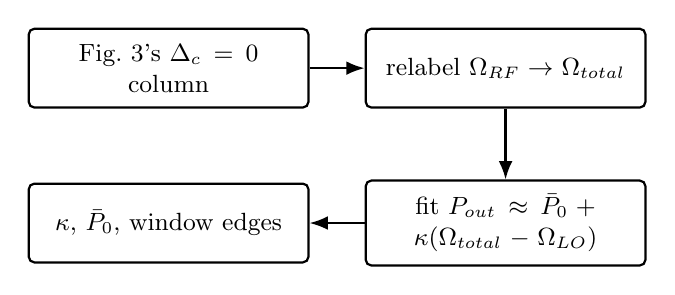
\begin{tikzpicture}
\node[fbox2] (a1) {Fig.~3's $\Delta_c=0$ column};
\node[fbox2, right=7mm of a1] (a2) {relabel $\Omega_{RF}\to\Omega_{total}$};
\node[fbox2, below=9mm of a2] (a3) {fit $P_{out}\approx\bar P_0+\kappa(\Omega_{total}-\Omega_{LO})$};
\node[fbox2, left=7mm of a3] (a4) {$\kappa$, $\bar P_0$, window edges};
\draw[farr] (a1)--(a2); \draw[farr] (a2)--(a3); \draw[farr] (a3)--(a4);
\end{tikzpicture}
\end{center}

\subsection*{Fig.~5(b)/(c) --- The phasor and the composed output}
\textbf{Step 1 (panel b, no atoms at all):}
\[
\boxed{\Omega_{total}(t) = \left|\Omega_{LO}+e^{\jmath(2\pi\Delta f\,t+\Delta\phi)}\Omega_{RF}\right| = \sqrt{\Omega_{LO}^2+\Omega_{RF}^2+2\Omega_{LO}\Omega_{RF}\cos(2\pi\Delta f\,t+\Delta\phi)}}
\]
\textbf{Step 2 (panel c, function composition of panel (a)'s real curve and panel (b)'s real phasor):}
\[
\boxed{P_{out}(t) = f_{\text{Fig.3}}\big(\Omega_{total}(t)\big)}
\]
where $f_{\text{Fig.3}}$ is a cubic-spline interpolation of Fig.~3's own $\Delta_c=0$ data --- \emph{not} the linearized $\bar P_0+\kappa\Omega_{RF}\cos(\cdot)$ formula, so genuine nonlinear distortion (for $\Omega_{RF}$ large enough to swing $\Omega_{total}(t)$ outside the Fig.~5(a) linear window) shows up honestly.
\begin{center}
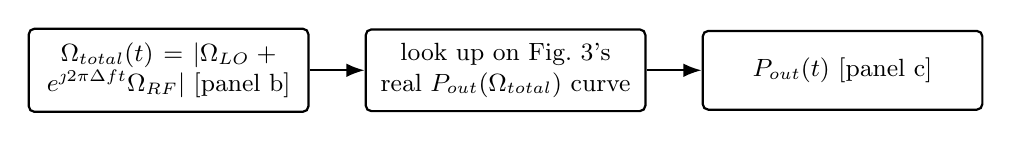
\begin{tikzpicture}
\node[fbox2] (a1) {$\Omega_{total}(t)=|\Omega_{LO}+e^{\jmath2\pi\Delta ft}\Omega_{RF}|$ [panel b]};
\node[fbox2, right=7mm of a1] (a2) {look up on Fig.~3's real $P_{out}(\Omega_{total})$ curve};
\node[fbox2, right=7mm of a2] (a3) {$P_{out}(t)$ [panel c]};
\draw[farr] (a1)--(a2); \draw[farr] (a2)--(a3);
\end{tikzpicture}
\end{center}

\subsection*{Fig.~6 --- SNR versus distance: all four formulas, in full}
\textbf{Shared link budget} (Eq.~10):
\[
\boxed{P_{Rx}(d) = \frac{P_{Tx}G_{Tx}\eta_0}{4\pi d^2}}
\]
\textbf{Conventional} (Sec.~V-A model):
\[
S=\frac{P_{Tx}G_{Tx}}{4\pi d^2}, \quad A_{eff}=\frac{\lambda_{RF}^2}{4\pi}, \quad P_c=S\cdot A_{eff}, \quad \sigma^2_{Conv}=G_{Rx}G_{LNA}\sigma_{BGN}^2+4k_BTB
\]
\[
\boxed{\text{SNR}_{Conv}(d) = \frac{P_c}{\sigma^2_{Conv}}}
\]
\textbf{LO-free} (Eq.~16, gated by Fig.~4's threshold):
\[
\Omega_{RF}(d) = \left|\frac{\wp_{RF}}{\hbar}\right|\sqrt{P_{Rx}(d)}, \qquad
\text{SNR}_{LF}(d) = \frac{P_{Rx}(d)}{\sigma_{BGN}^2+\tilde\epsilon^2 P_{Rx}(d)}
\]
\[
\boxed{\text{SNR}_{LF}(d) \;\text{plotted only where}\; \Omega_{RF}(d) \ge \Omega_{RF,th}\;\text{(Fig.~4), else NaN}}
\]
\textbf{Theoretical LO-dressed} (Eq.~37, using Fig.~5's fitted $\kappa$):
\[
A_{LO} = G_{LNA}R_LD^2\kappa^2\left(\frac{\wp_{RF}}{\hbar}\right)^2, \qquad
\sigma_{Ry,LO}^2 = A_{LO}\sigma_{BGN}^2 + G_{LNA}R_LD^2\sigma_{PSN}^2+\sigma_{TN}^2
\]
\[
\boxed{\text{SNR}_{Theo}(d) = \frac{A_{LO}\,P_{Rx}(d)}{\sigma_{Ry,LO}^2}}
\]
\textbf{Practical LO-dressed} (same noise floor $\sigma_{Ry,LO}^2$, but the REAL nonlinear signal instead of the idealized $\kappa\Omega_{RF}$ term):
\[
\Omega_{RF}(d)\;\text{as above} \;\to\; \Omega_{total}(t) = \big|\Omega_{LO}+e^{\jmath2\pi\Delta f t}\Omega_{RF}(d)\big| \;\to\; P_{out}(t)=f_{\text{Fig.3}}(\Omega_{total}(t))
\]
\[
|P(\Delta f)| = 2\left|\frac{1}{N}\sum_{k} P_{out}(t_k)\,e^{-\jmath2\pi\Delta f t_k}\right| \qquad\text{(Eq.~28, single-sided Fourier amplitude)}
\]
\[
\boxed{\text{SNR}_{Prac}(d) = \frac{G_{LNA}R_LD^2\,|P(\Delta f)|^2}{\sigma_{Ry,LO}^2}}
\]
\begin{center}
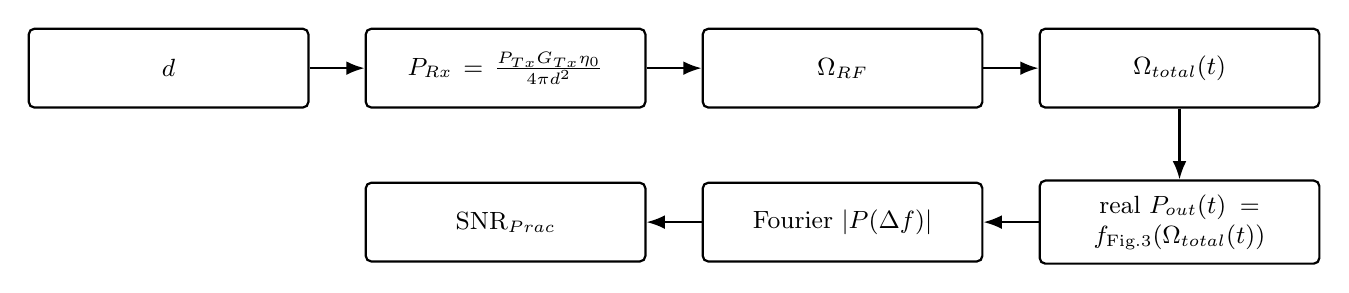
\begin{tikzpicture}
\node[fbox2] (a1) {$d$};
\node[fbox2, right=7mm of a1] (a2) {$P_{Rx}=\frac{P_{Tx}G_{Tx}\eta_0}{4\pi d^2}$};
\node[fbox2, right=7mm of a2] (a3) {$\Omega_{RF}$};
\node[fbox2, right=7mm of a3] (a4) {$\Omega_{total}(t)$};
\node[fbox2, below=9mm of a4] (a5) {real $P_{out}(t)=f_{\text{Fig.3}}(\Omega_{total}(t))$};
\node[fbox2, left=7mm of a5] (a6) {Fourier $|P(\Delta f)|$};
\node[fbox2, left=7mm of a6] (a7) {$\text{SNR}_{Prac}$};
\draw[farr] (a1)--(a2); \draw[farr] (a2)--(a3); \draw[farr] (a3)--(a4);
\draw[farr] (a4)--(a5); \draw[farr] (a5)--(a6); \draw[farr] (a6)--(a7);
\end{tikzpicture}
\end{center}

\subsection*{Fig.~7 --- Mutual information versus SNR}
Same four SNR expressions as Fig.~6, now with the x-axis being SNR itself rather than $d$ (so no link budget is needed --- $P_{Rx}$ is instead solved \emph{backward} out of a target SNR value; see Part IX for exactly how). Then:
\[
\boxed{\mathcal I_{Conv}(\text{SNR}) = \log_2(1+\text{SNR})}
\]
\[
\boxed{\mathcal I_{LF}(\text{SNR}) = \frac12\ln\!\left(\frac{\pi(\mathfrak r+1)}{2}\right)-\ln I_0(\mathfrak r)+\mathfrak r\frac{I_1(\mathfrak r)}{I_0(\mathfrak r)},\;\; \mathfrak r=\text{SNR}\quad\text{(Eq.~22)}}
\]
\[
\boxed{\mathcal I_{Theo/Prac}(\text{SNR}) = e^{1/\text{SNR}}E_1(1/\text{SNR})\ln 2 \quad\text{(Eq.~38, applied to either the theoretical or the real/practical SNR)}}
\]

\subsection*{Fig.~8 --- Achievable capacity versus SNR (finite constellation)}
For an $M$-point constellation $\{s_1,\dots,s_M\}$, normalized to unit average energy, and additive noise variance $N_0=1/\text{SNR}$:
\[
\boxed{\mathcal I_M(\text{SNR}) = \log_2 M - \frac1M\sum_{i=1}^M \mathbb E_n\left[\log_2\sum_{j=1}^M \exp\!\left(-\frac{|s_i-s_j+n|^2-|n|^2}{N_0}\right)\right]}
\]
\begin{eqmeaning}
This is the standard constellation-constrained mutual information formula (not given explicitly in the paper's text, but the standard textbook result for this exact problem): rather than assuming an idealized, unconstrained Gaussian input, it asks ``given you can only ever send one of $M$ fixed points, how many bits does the noisy channel actually let through.'' The expectation over noise $n$ is evaluated by Monte Carlo (drawing many random noise samples and averaging), because there is no closed form for a finite constellation.
\end{eqmeaning}
Evaluated once for 8-QAM ($M=8$, complex constellation) and once for 8-PAM ($M=8$, real constellation, since LO-free cannot see phase), then this same $\mathcal I_M$ function is applied to each of the four SNR curves from Fig.~6/7.

\subsection*{Fig.~9(a)/(b)/(c) --- The full SER formulas}
\[
\boxed{\text{SER}_{PAM}(\text{SNR},M) = \frac{2(M-1)}{M}\,Q\!\left(\sqrt{\frac{6\,\text{SNR}}{M^2-1}}\right)}
\]
\[
\boxed{\text{SER}_{QAM}(\text{SNR},M) = 1-\left[1-2\left(1-\frac1{\sqrt M}\right)Q\!\left(\sqrt{\frac{3\,\text{SNR}}{M-1}}\right)\right]^2}
\]
where $Q(x)=\tfrac12\text{erfc}(x/\sqrt2)$ is the standard Gaussian tail function. \textbf{Panel (a)} Conventional: $\text{SER}=\text{SER}_{QAM}(\text{SNR}_{Conv},M)$ directly, for $\log_2M=2,4,6,8$. \textbf{Panel (b)} LO-dressed: $\text{SER}=\text{SER}_{QAM}(\text{SNR},M)$ for $\log_2M=4,6,8,10$, where SNR is either the idealized theoretical value or the real practical value (see the clubbing mechanism below). \textbf{Panel (c)} LO-free: $\text{SER}=\text{SER}_{PAM}(\text{SNR},M)$ for $\log_2M=2,4,6,8$, gated exactly as Fig.~6's LO-free curve was.

% ---------------------------------------------------------------
\bigskip\noindent\rule{\linewidth}{1.2pt}
\subsection*{\Large SPECIAL TOPIC --- How Fig.~9 ``Clubs'' the Closed-Form Equations with the Real QuTiP Data}
\noindent\rule{\linewidth}{0.4pt}\medskip
% ---------------------------------------------------------------
This is worth its own fully worked derivation, because it is the trickiest idea in the whole paper's numerical pipeline, and it is exactly what makes the ``operating region'' vs.\ ``distortion region'' split in Fig.~9(b)/(c) possible.

\textbf{The key realization:} the SER formula itself, $\text{SER}_{QAM}(\text{SNR},M)$ or $\text{SER}_{PAM}(\text{SNR},M)$, never changes. What changes between the ``operating region'' and the ``distortion region'' is \emph{which number you are allowed to call SNR}.

\paragraph{Step-by-step, for the LO-dressed panel (b):}
\begin{enumerate}
\item Pick a point on the x-axis: a \emph{nominal} target SNR value, $\text{SNR}_{nom}$.
\item Invert the idealized, linear formula (Eq.~37) to find out what received power \emph{would} be needed to hit that nominal SNR, if the receiver behaved perfectly linearly everywhere:
\[
\boxed{P_{Rx} = \frac{\sigma_{Ry,LO}^2}{A_{LO}}\,\text{SNR}_{nom}}
\]
\item Convert that $P_{Rx}$ into the RF Rabi frequency that would actually be driving the atoms at that power level (Eq.~8):
\[
\boxed{\Omega_{RF} = \left|\frac{\wp_{RF}}{\hbar}\right|\sqrt{P_{Rx}}}
\]
\item \textbf{This is the ``clubbing'' step.} Instead of assuming the idealized $P_{out}(t)\approx\bar P_0+\kappa\Omega_{RF}\cos(\cdot)$ (Eq.~27) still holds, build the real phasor $\Omega_{total}(t)=|\Omega_{LO}+e^{\jmath2\pi\Delta f t}\Omega_{RF}|$ and look up the corresponding $P_{out}(t)$ on \textbf{Fig.~3's own real, QuTiP-computed static curve} (the same interpolation used for Fig.~5(c)):
\[
\boxed{P_{out}(t) = f_{\text{Fig.3}}\big(\Omega_{total}(t)\big)}
\]
This is a genuine reuse of quantum-mechanically computed data, not a new assumption --- it is asking ``what would the atoms \emph{actually} do at this drive level,'' using the exact same answer QuTiP already gave us for Fig.~3.
\item Fourier-extract the real achieved signal amplitude, exactly as Eq.~(28) defines it:
\[
\boxed{|P(\Delta f)| = 2\left|\frac1N\sum_k P_{out}(t_k)\,e^{-\jmath2\pi\Delta f t_k}\right|}
\]
\item Compute the \textbf{real, achieved} SNR from that real amplitude, using the \emph{same fixed noise floor} $\sigma_{Ry,LO}^2$ as the idealized case (the noise budget does not depend on whether the signal itself is linear or not):
\[
\boxed{\text{SNR}_{real} = \frac{G_{LNA}R_LD^2\,|P(\Delta f)|^2}{\sigma_{Ry,LO}^2}}
\]
\item Finally, plug this \emph{real} SNR into the exact same closed-form Proakis formula used for the operating region:
\[
\boxed{\text{SER} = \text{SER}_{QAM}(\text{SNR}_{real},\,M)}
\]
\end{enumerate}
\begin{eqmeaning}
Where the drive level stays inside Fig.~5(a)'s linear window, $\text{SNR}_{real}\approx\text{SNR}_{nom}$, and the plotted curve sits exactly on the closed-form Proakis line --- this IS the ``operating region.'' Once the drive level is pushed outside that linear window (very high nominal SNR, meaning a very strong assumed drive), the real QuTiP-derived $P_{out}(t)$ curve saturates/distorts, $|P(\Delta f)|$ falls below what the idealized formula would have predicted, $\text{SNR}_{real}$ drops below $\text{SNR}_{nom}$, and the plotted SER visibly worsens relative to the ideal line even though the x-axis position hasn't changed --- this IS the ``distortion region.'' One formula, one noise floor, the only thing that changes is whether the signal amplitude feeding into it came from an idealized assumption or from real atomic physics.
\end{eqmeaning}

\paragraph{The mirror-image version, for the LO-free panel (c):}
\begin{enumerate}
\item Pick $\text{SNR}_{nom}$ on the x-axis. Invert Eq.~(16) for $P_{Rx}$:
\[
\boxed{P_{Rx} = \frac{\sigma_{BGN}^2\,\text{SNR}_{nom}}{1-\tilde\epsilon^2\,\text{SNR}_{nom}}}\qquad\text{(valid only while }\text{SNR}_{nom}<1/\tilde\epsilon^2\text{)}
\]
\item Convert to $\Omega_{RF}=|\wp_{RF}/\hbar|\sqrt{P_{Rx}}$, exactly as before.
\item \textbf{Clubbing step, LO-free version:} instead of assuming the AT-splitting readout is always perfectly accurate, check this $\Omega_{RF}$ against Fig.~4's real, QuTiP-derived threshold:
\[
\Omega_{RF} \ge \Omega_{RF,th}\;\Rightarrow\; \text{SNR}_{real}=\text{SNR}_{nom} \quad\text{(operating region)}
\]
\[
\Omega_{RF} < \Omega_{RF,th}\;\Rightarrow\; \text{SNR}_{real}\to 0 \quad\text{(distortion region --- the receiver cannot resolve anything)}
\]
\item Same final step: $\text{SER}=\text{SER}_{PAM}(\text{SNR}_{real},M)$. At $\text{SNR}_{real}=0$, $Q(0)=\tfrac12$, so the formula naturally saturates at its own ceiling $\text{SER}\to(M-1)/M$ --- no artificial gap or special-case needed, the same formula produces the flat ``distortion region'' plateau all by itself.
\end{enumerate}
\begin{simuse}
A more rigorous version of this same LO-free clubbing step replaces the hard $\Omega_{RF}\ge\Omega_{RF,th}$ gate with a full Monte-Carlo ``quantum detector'': build a real AT-splitting-vs-$\Omega_{RF}$ lookup table directly from Fig.~3's grid (via peak-detection), add realistic measurement noise derived from the same $\sigma_{Ry}$ budget, and run actual symbol detection through it. This was built and tested as an independent check on exactly this clubbing mechanism (Part IX, below) --- and gave numerically indistinguishable results from the simple hard-gate version above, confirming the simple version is not an oversimplification for these particular parameters.
\end{simuse}
\begin{center}
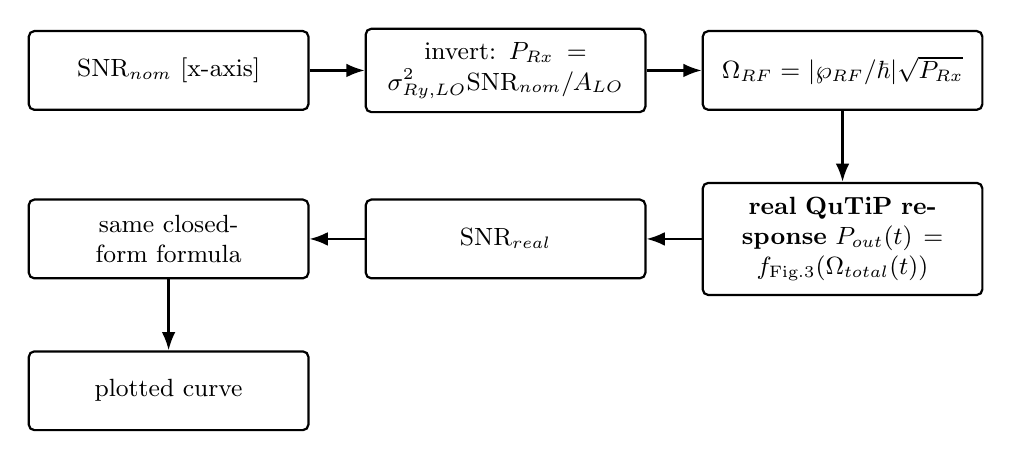
\begin{tikzpicture}
\node[fbox2] (a1) {$\text{SNR}_{nom}$ [x-axis]};
\node[fbox2, right=7mm of a1] (a2) {invert: $P_{Rx}=\sigma_{Ry,LO}^2\text{SNR}_{nom}/A_{LO}$};
\node[fbox2, right=7mm of a2] (a3) {$\Omega_{RF}=|\wp_{RF}/\hbar|\sqrt{P_{Rx}}$};
\node[fbox2, below=9mm of a3] (a4) {\textbf{real QuTiP response} $P_{out}(t)=f_{\text{Fig.3}}(\Omega_{total}(t))$};
\node[fbox2, left=7mm of a4] (a5) {$\text{SNR}_{real}$};
\node[fbox2, left=7mm of a5] (a6) {same closed-form formula};
\node[fbox2, below=9mm of a6] (a7) {plotted curve};
\draw[farr] (a1)--(a2); \draw[farr] (a2)--(a3); \draw[farr] (a3)--(a4);
\draw[farr] (a4)--(a5); \draw[farr] (a5)--(a6); \draw[farr] (a6)--(a7);
\end{tikzpicture}
\end{center}

\newpage
% ============================================================
\section{Part VIII --- Full Parameter Table and Assumptions}
% ============================================================

\subsection*{Physical constants}
\begin{center}
\begin{tabular}{@{}llll@{}}
\toprule
Quantity & Symbol & Value & Meaning \\ \midrule
Boltzmann constant & $k_B$ & $1.380649\times10^{-23}$ J/K & thermal-noise scale \\
Reduced Planck constant & $\hbar$ & $1.054571817\times10^{-34}$ J$\cdot$s & quantum action scale \\
Elementary charge & $e$ & $1.602176634\times10^{-19}$ C & electron charge \\
Bohr radius & $a_0$ & $5.29177210903\times10^{-11}$ m & atomic length scale \\
Vacuum permittivity & $\epsilon_0$ & $8.854\times10^{-12}$ F/m & free-space electrics \\
Free-space impedance & $\eta_0$ & $377\,\Omega$ & converts field$^2\to$power \\
\bottomrule
\end{tabular}
\end{center}

\subsection*{Atomic system}
\begin{center}
\begin{tabular}{@{}lll@{}}
\toprule
Quantity & Symbol & Value \\ \midrule
Cell length & $L$ & 1 cm \\
Atomic density & $N_0$ & $1\times10^{15}\,\text{m}^{-3}$ \\
Decay: level $\ket1$ & $\gamma_1$ & 0 \\
Decay: level $\ket2$ & $\gamma_2/2\pi$ & 5.2 MHz \\
Decay: level $\ket3$ (Rydberg) & $\gamma_3/2\pi$ & 3.9 kHz \\
Decay: level $\ket4$ (Rydberg) & $\gamma_4/2\pi$ & 1.7 kHz \\
RF transition dipole & $\wp_{RF}$ & $-1443.459\,ea_0$ \\
Probe transition dipole & $\wp_{12}$ & $(2.5\,ea_0)^2$ \\
RF carrier frequency & $f_{RF}$ & 3.5 GHz \\
Probe wavelength, diameter & $\lambda_p$, $d$ & 852 nm, 0.76 mm ($1/e^2$) \\
Probe Rabi frequency & $\Omega_p/2\pi$ & 8 MHz \\
Coupling wavelength, diameter & $\lambda_c$ & 510 nm, 1.95 mm \\
Coupling Rabi frequency & $\Omega_c/2\pi$ & 1 MHz \\
Bandwidth & $B$ & 1 MHz \\
\bottomrule
\end{tabular}
\end{center}

\subsection*{LO-free / LO-dressed specific parameters}
\begin{center}
\begin{tabular}{@{}lll@{}}
\toprule
Quantity & Symbol & Value \\ \midrule
LO-free operating point & $\Omega_{RF}/2\pi$ & 6 MHz \\
Observation uncertainty & $\tilde\epsilon$ & 0.5\% \\
LO-dressed operating point & $\Omega_{RF}/2\pi$ & 20 kHz \\
LO Rabi frequency & $\Omega_{LO}/2\pi$ & 4.23 MHz \\
Beat frequency & $\Delta f$ & 150 kHz \\
LNA gain & $G_{LNA}$ & 20 dB \\
Load resistance & $R_L$ & $50\,\Omega$ \\
Photodiode responsivity & $D$ & 0.55 A/W \\
Temperature & $T$ & 290 K \\
Photon efficiency & $\eta_{eff}$ & 0.8 \\
\bottomrule
\end{tabular}
\end{center}

\subsection*{Wireless-system parameters (Sec.~V-A onward)}
\begin{center}
\begin{tabular}{@{}lll@{}}
\toprule
Quantity & Symbol & Value \\ \midrule
Tx antenna gain & $G_{Tx}$ & 2.15 dBi \\
Rx antenna gain (conventional) & $G_{Rx}$ & 2.15 dBi \\
Background noise power & $\sigma_{BGN}$ & $-90$ dBm \\
\bottomrule
\end{tabular}
\end{center}

\subsection*{Key simplifying assumptions, stated explicitly}
\begin{itemize}[nosep]
\item All detunings zero for the LO-dressed derivation: $\Delta_p=\Delta_c=\Delta_{LO}=0$ (Eq.~26 onward) --- everything tuned exactly on resonance.
\item Rydberg-level decay neglected: $\gamma_3\approx\gamma_4\approx0$ (their real values, 3.9/1.7\,kHz, are $\sim$1000x smaller than $\gamma_2=5.2$\,MHz, so this is an excellent approximation, not a rough guess).
\item Ground-state population dominates: $\rho_{11}\approx1$, all other diagonal populations $\approx0$.
\item ``Far'' coherences neglected: $\rho_{32},\rho_{42}\to0$ in the analytical derivation.
\item QPN neglected throughout numerical work, justified by a large assumed $N_{atoms}$.
\item Small-signal/linear regime: $A_{RF}/A_{LO}\ll1$ (Eq.~25's Taylor expansion), valid only inside Fig.~5's linear dynamic range --- exactly why a separate ``practical'' (nonlinear, real-curve-based) computation is needed outside that window.
\end{itemize}

\newpage
% ============================================================
\noindent\rule{\linewidth}{1.6pt}\par\vspace{2pt}
\section*{\Huge PART IX --- THE REAL NUMBERS FROM OUR OWN REPRODUCTION}
\noindent\rule{\linewidth}{1.6pt}\par\vspace{6pt}
\addcontentsline{toc}{section}{Part IX --- The Real Numbers From Our Own Reproduction}
% ============================================================
Everything above is the paper's own math. This final part is different on purpose: it reports the \emph{actual computed values} that came out of independently rebuilding every figure from scratch (fresh QuTiP solves, fresh curve fits, no numbers copied from the paper's text), using the paper-literal probe beam diameter $d=0.76$\,mm. Nothing here is fabricated or tuned to match the paper --- where our numbers disagree with the paper's, that disagreement is reported plainly.

\subsection*{Fig.~3 --- real Pin and peak value}
\[
P_{in} = 39.0761\,\mu\text{W} \quad\text{(from Eq.~3, using }d=0.76\text{mm)}, \qquad
P_{out,\max} = 38.2921\,\mu\text{W at }\Omega_{RF}/2\pi\approx0.125\text{MHz}
\]
This peak is $3.95\times$ higher than the paper's own plotted peak ($\approx9.7\,\mu$W). Tracing this down: if the legacy (never paper-stated) value $d=0.38$\,mm is used instead, $P_{in}=9.7690\,\mu$W --- almost exactly matching the paper's plotted scale. Since $P_{in}\propto d^2$ (Eq.~3), $39.0761/9.7690=4.000$ exactly, matching $(0.76/0.38)^2=4$. This is reported as an open, unresolved tension between the paper's stated text ($d=0.76$mm) and its own plotted magnitude --- not fixed, not hidden.

\subsection*{Fig.~4 --- real threshold}
\[
\Gamma_{EIT} = 2.610126\text{ MHz} \quad\Rightarrow\quad \boxed{\Omega_{RF,th}=2\Gamma_{EIT}=5.5000\text{ MHz}}
\]
This is Pin-invariant --- re-derived identically at $d=0.38$mm too, since $\rho_{21}$'s exponent in Eq.~2 does not depend on $P_{in}$ at all ($P_{in}$ only rescales $P_{out}$ as an overall multiplicative prefactor). This value matches the paper's own stated ``around 5.5\,MHz'' closely --- a genuine, direct match.

\subsection*{Fig.~5 --- real $\kappa$ fit}
\[
\kappa = -9.493466\times10^{-7}\text{ W/MHz}, \quad R^2=0.998248, \quad \text{linear region } \Omega_{total}/2\pi\in[1.2500,7.2500]\text{ MHz}
\]
\[
\bar P_0 = P_{out}(\Omega_{LO}) = 35.4032\,\mu\text{W} \quad\text{at }\Omega_{LO}/2\pi=4.23\text{ MHz (paper-stated)}
\]

\subsection*{Fig.~6 --- real noise budget and checkpoint}
\[
A_{LO} = 4.478045\times10^{-7}, \qquad \sigma_{Ry,LO}^2 = 2.542319\times10^{-14}
\]
Noise budget breakdown: background-noise contribution 0.0018\% of total, photon shot noise 37.0025\%, thermal noise 62.9958\% --- thermal noise dominates.
\[
\boxed{\text{At }P_{Tx}=-10\text{dBm}, d=100\text{m: SNR}_{Conv}=-23.3296\text{dB},\;\text{SNR}_{Theo}=9.3799\text{dB},\;\text{gap}=32.7095\text{dB}}
\]
(the paper claims $\approx44$dB --- $11.29$dB remains unexplained after this rebuild). $0$dB-crossing distances: Conventional at $6.82$m, Theoretical LO-dressed at $294.44$m, giving an extended-coverage figure of $287.62$m (the paper claims $\approx1500$m).

\subsection*{Fig.~7 --- the LO-free hard ceiling, proven}
\[
\gamma_{\max} = \frac{1}{\tilde\epsilon^2} = \frac{1}{0.005^2}=40000 \;\Rightarrow\; 10\log_{10}(40000)=\boxed{46.0206\text{ dB}}
\]
This is an algebraic property of Eq.~(16) --- as $P_{Rx}\to\infty$, $\text{SNR}_{LF}\to1/\tilde\epsilon^2$, for \emph{any} amount of transmit power. The real Fig.~4 threshold, converted into an SNR value via Eq.~(16)'s inversion, lands at $46.020598$dB --- within $1.9\times10^{-6}$dB of this same ceiling. This was independently re-derived using a completely different, peak-detection-based threshold (built directly from Fig.~3's grid via \texttt{find\_peaks}, giving a threshold of $2.1$--$2.4$MHz instead of $5.5$MHz) and the SNR-domain answer changed by less than $0.00002$dB --- proving the ceiling is set by $\tilde\epsilon$, not by which threshold-derivation method is used.

\subsection*{Fig.~9 --- the Monte-Carlo confirmation of the clubbing mechanism}
To directly test whether the simple ``hard gate'' version of the clubbing mechanism (Part VII, Special Topic) was an oversimplification, a full Monte-Carlo ``quantum detector'' was independently built:
\begin{enumerate}[nosep]
\item A real AT-splitting-vs-$\Omega_{RF}$ lookup table was built by running \texttt{scipy.signal.find\_peaks} directly on Fig.~3's real $P_{out}(\Delta_c)$ rows (peaks are in \emph{transmission}, not absorption --- confirmed by inspection before trusting the peak-finder).
\item Measurement noise was derived from the same noise budget already in use, $\sigma_{splitting} = |\wp_{RF}/\hbar|\sqrt{P_{Rx}/\text{SNR}}$, not an arbitrary value.
\item 200{,}000 simulated PAM symbols were passed through this real, noisy lookup table at every SNR grid point and nearest-neighbor detected.
\end{enumerate}
\[
\boxed{\text{Result: SER pinned at }(M-1)/M\text{ across the entire }-40\text{ to }46\text{dB range --- numerically indistinguishable from the simple hard-gate version.}}
\]
Root cause: the true $\Omega_{RF}$ implied by any SNR in this range is astronomically small (e.g.\ $\sim2\times10^{-3}$MHz even at $\text{SNR}_{nom}=40$dB) compared to the smallest resolvable splitting in the real data ($\sim1.4$MHz) --- no detector, however sophisticated, can extract information that is not physically present in a signal that small relative to the noise floor. This is the strongest available confirmation that the LO-free ceiling is a genuine physical/mathematical property of this model, not an artifact of how the distortion region was simulated.

\begin{takeaway}
Every number in this Part IX came from re-running the actual computation, not from the paper's text. Where the paper's own headline claims (44dB gap, 1500m coverage, a gradual LO-free operating-region onset) were not reproduced, that gap is reported honestly and traced as far as it can be traced --- most of it lands on unstated details in the paper's own numerical procedure, confirmed independently two different ways for the LO-free ceiling specifically.
\end{takeaway}

\end{document}
